%
% Exemplo LaTeX de artigo UNISINOS
%
% Elaborado com base nas orientações dadas no documento
% ``GUIA PARA ELABORAÇÃO DE TRABALHOS ACADÊMICOS''
% disponível no site da biblioteca da Unisinos.
% http://www.unisinos.br/biblioteca
%
% Os elementos textuais abaixo são apresentados na ordem em que devem
% aparecer no documento.  Repare que nem todos são obrigatórios - isso
% é devidamente indicado em cada caso.
%
% Comentários abaixo colocados entre aspas (`` '') foram
% extraídos diretamente do documento da biblioteca.
%
% Este documento é de domínio público.
%

%=======================================================================
% Declarações iniciais identificando a classe de documento e
% selecionando alguns pacotes adicionais.
%
% As opções disponíveis (separe-as com vírgulas, sem espaço) são:
% - twoside: Formata o documento para impressão frente-e-verso
%   (o default é somente-frente)
% - english,brazilian,french,german,etc.: idiomas usados no documento.
%   Deve ser colocado por último o idioma principal.
%=======================================================================
\documentclass[oneside,brazilian,english]{UNISINOSartigo}
\usepackage[utf8]{inputenc} % charset do texto (utf8, latin1, etc.)
\usepackage[T1]{fontenc} % encoding da fonte (afeta a sep. de sílabas)
\usepackage{graphicx} % comandos para gráficos e inclusão de figuras
\usepackage{bibentry} % para inserir refs. bib. no meio do texto

%=======================================================================
% Escolha do sistema para geração de referências bibliográficas.
%
% O default é usar o estilo unisinos.bst.  Comente a definição abaixo
% e descomente a linha seguinte para usar o estilo do ABNTeX (é
% necessário ter esse pacote instalado).
%
% A vantagem do unisinos.bst é que ele permite o uso de um arquivo .bib
% seguindo as orientações tradicionais do BibTeX (veja essas orientações
% em http://ctan.tug.org/tex-archive/biblio/bibtex/contrib/doc/btxdoc.pdf).
% Entretanto, o estilo não suporta algumas citações mais exóticas como
% apud.  Para isso, use o ABNTeX, mas esteja ciente de que muitas de
% suas referências serão incompatíveis com os estilos tradicionais do
% BibTeX como plain, alpha, ieeetr, entre outros.
%=======================================================================
\unisinosbst
%\usepackage[alf]{abntcite}
\usepackage{hyperref} 
\usepackage{booktabs}
\usepackage{graphicx}

\usepackage{listings}
\usepackage{color}
\usepackage{pdflscape}

\definecolor{dkgreen}{rgb}{0,0.6,0}
\definecolor{gray}{rgb}{0.5,0.5,0.5}
\definecolor{mauve}{rgb}{0.58,0,0.82}

\lstset{frame=tb,
  language=Python,
  aboveskip=3mm,
  belowskip=3mm,
  showstringspaces=false,
  columns=flexible,
  basicstyle={\small\ttfamily},
  numbers=none,
  numberstyle=\tiny\color{gray},
  keywordstyle=\color{blue},
  commentstyle=\color{dkgreen},
  stringstyle=\color{mauve},
  breaklines=true,
  breakatwhitespace=false,
  escapechar=@,
  tabsize=2,
  breakindent=2ex,
  postbreak=\raisebox{0ex}[0ex][0ex]{\ensuremath{\hookrightarrow\space}}
}



%=======================================================================
% Informações Pessoais
%=======================================================================
\title{Using Word embeddings for word similarity identification in Brazilian Portuguese}
\othertitle{Usando o Word Embeddings para identificação de similaridade de palavras no português brasileiro}

\author{Eduardo Eidelwein Berlitz}
\authorinfo{Aluno do curso de Ciência da Computação. Email: eberlitz@gmail.com}
\degree{Bacharel em Ciência da Computação}
\course{Curso de Ciência da Computação}
\address{São Leopoldo}
\date{2018}

\advisor[Prof. Dr.]{Sandro José Rigo}
\advisorinfo{Orientador, professor da Unisinos. Email: rigo@unisinos.br}
% \advisorinfo{Orientador, professor da Unisinos, doutor em Ciência da Computação pela Universidade de Stanford (1995), Mestre em Ciência da Computação pela Universidade de Calcutá (1983). Email: professor@unisinos.br}

\coadvisor[Prof.~PhD.]{Rodrigo da Rosa Righi}
\coadvisorinfo{Coorientador, professor da Unisinos. Email: rrrighi@unisinos.br}
%=======================================================================
% Início do documento.
%=======================================================================
\begin{document}

\maketitle


% \begin{otherlanguage}{brazilian}
%   % \begin{abstract}
%   % A capacidade de identificar a similaridade semântica entre palavras tem sido objeto de pesquisa nos últimos anos, pois está relacionada a uma série de atividades da área de processamento de linguagem natural, como recuperação de informação, sumarização de texto, categorização e geração, tradução automática e outros. A maioria dos sistemas de resposta a perguntas e extração de informações usa o WordNet para procurar sinônimos em seu mecanismo de busca. No entanto, a expansão de termos usando o WordNet tem vários problemas. Eles são de construção manual, demorados e caros, e por esse motivo, nem todos os links estarão presentes e sua qualidade varia de idioma para idioma, assim como não está disponível para todos os idiomas. Abordagens baseadas em distribuição, como a \textit{word embedding}, foram usadas para cobrir itens fora do vocabulário no WordNet. Assim, com a possibilidade de acesso a diferentes \textit{word embeddings models} e a necessidade de melhorar a forma de expandir os termos relacionados aos sistemas de consulta para bases ontológicas utilizadas por sistemas de perguntas e respostas e recuperação de informação, o presente trabalho explora as técnicas existentes para identificação de similaridade entre palavras, usando a abordagem distribuicional chamada word embeddings, adaptandando trabalhos existentes para o português brasileiro. Também é realizado experiementos com outras tecnicas que são basesadas em bases lexicas como WordNet, aonde uma avaliação qualitativa é realizada de todas as técnicas sobre um \textit{dataset} comun PT65. Provando que word embeddings podem de fato cobrir as palavras faltantes e tem um resultado ligeiramente melhor quando comparado com o WordNet. Também é realizado uma adaptação de estudos sobre a adição do contexto sintático no processo de trainamento do word embeddings a partir e um corpus português brasileiro, aonde obtivemos resultados similares atraves de uma avaliação qualitativa, porem para a atividade de identificar palavras similares utilizando o dataset PT65 os resultados foram piores em considersão aos outros modelos.
%   % \palavraschave{Similaridade de palavras. WordNet. Word embedding. Linguística computacional. Processamento de Linguagem Natural.}
%   % \end{abstract}
% \end{otherlanguage}
  


%=======================================================================
% Resumo em Português.
%
% A recomendação é para 150 a 250 palavras.
%=======================================================================
%=======================================================================
% Resumo em Português.
%
% A recomendação é para 150 a 500 palavras.
%=======================================================================
\begin{abstract}
The ability to identify the semantic similarity between words has been a subject of research very explored in the last years, because it is related to a series of activities of the area of natural language processing like information retrieval, text summarization, categorization and generation, database schema matching, question answering, machine translation, and others. Most of question answering and information extraction systems use WordNet to search for synonyms in their search engine. However, the expansion of terms using WordNet has several problems. They are of manual construction, time-consuming and expensive, and for this reason, not all links will be present and their quality varies from language to language, as also, it is not available for all languages. Distributional-based approaches like word embeddings have successfully been used to cover out-of-vocabulary items in WordNet. Thus, with the possibility of access to different word embeddings models and the need to improve the way of expanding related terms of query systems to ontological bases used by systems of questions answering and information retrieval, the present work explores the existing techniques regarding word similarity, using a distributional approach called word embeddings, adapting existing works to Brazilian Portuguese. We also experiment with other techniques that are solely based on a lexical database such as WordNet, and we do a qualitative evaluation of all the different techniques over a common dataset called PT65. Proving that word embeddings can cover words out of vocabulary and have slightly better results in comparison with WordNet. We also adapted the studies regarding the addition of syntactic context in the training process of word embeddings to a Brazilian Portuguese corpus, finding similar results through a qualitative evaluation, but for the task of word similarity against the dataset PT65, it had the worst results.
\palavraschave{Word similarity. WordNet. Word embedding. Computational linguistics. Natural Language Processing.}
\end{abstract}

%=======================================================================
% Resumo em língua estrangeira (sim, é aqui mesmo).
%
% O idioma usado aqui deve necessariamente aparecer nos parâmetros do
% \documentclass, no início do documento.
%=======================================================================
\begin{otherlanguage}{brazilian}
    % \othertitle{Utilizando Word Embeddings para similaridade de palavras no Português Brasileiro}
\begin{abstract}
A capacidade de identificar a similaridade semântica entre palavras tem sido objeto de pesquisa nos últimos anos, pois está relacionada a uma série de atividades da área de processamento de linguagem natural, como recuperação de informação, sumarização de texto, categorização e geração, tradução automática e outros. A maioria dos sistemas de resposta a perguntas e extração de informações usa o WordNet para procurar sinônimos em seu mecanismo de busca. No entanto, a expansão de termos usando o WordNet tem vários problemas. Eles são de construção manual, demorados e caros, e por esse motivo, nem todos os links estarão presentes e sua qualidade varia de idioma para idioma, assim como não está disponível para todos os idiomas. Abordagens baseadas em distribuição, como a \textit{word embedding}, foram usadas para cobrir itens fora do vocabulário no WordNet. Assim, com a possibilidade de acesso a diferentes \textit{word embeddings models} e a necessidade de melhorar a forma de expandir os termos relacionados aos sistemas de consulta para bases ontológicas utilizadas por sistemas de perguntas e respostas e recuperação de informação, o presente trabalho explora as técnicas existentes para identificação de similaridade entre palavras, usando a abordagem distribuicional chamada word embeddings, adaptandando trabalhos existentes para o português brasileiro. Também é realizado experiementos com outras tecnicas que são basesadas em bases lexicas como WordNet, aonde uma avaliação qualitativa é realizada de todas as técnicas sobre um \textit{dataset} comun PT65. Provando que word embeddings podem de fato cobrir as palavras faltantes e tem um resultado ligeiramente melhor quando comparado com o WordNet. Também é realizado uma adaptação de estudos sobre a adição do contexto sintático no processo de trainamento do word embeddings a partir e um corpus português brasileiro, aonde obtivemos resultados similares atraves de uma avaliação qualitativa, porem para a atividade de identificar palavras similares utilizando o dataset PT65 os resultados foram piores em considersão aos outros modelos.
\palavraschave{Similaridade de palavras. WordNet. Word embedding. Linguística computacional. Processamento de Linguagem Natural.}
\end{abstract}
\end{otherlanguage}


%=======================================================================
% Introdução
%=======================================================================

% G
\section{Introduction}\label{chap:intro}

Natural Language Processing (NLP) is a field whose purpose is to make computers perform tasks using human languages. In these systems, a series of components must be studied as speech recognition, natural language understanding, and speech synthesis. According to \citetexto[p.~29]{Jurafsky:2009:SLP:1214993}, "What distinguishes language processing applications from other data processing systems is their use of \textit{knowledge of language}.". That is, for several NLP activities you need knowledge about phonetics, phonology, morphology, lexical semantics, compositional semantics. \cite{Jurafsky:2009:SLP:1214993}.

The ability to identify the semantic similarity between words has been a subject of research explored in the last years, because it is related to a series of activities of the area of natural language processing like information retrieval, text summarization, categorization and generation, database schema matching, question answering, machine translation, and others. \cite{Pawar2018CalculatingTS, SRAVANTHI2017SemanticSB, Islam2007ApplicationsOC}. 

% --------------------------------------------------------------
\subsection{Motivation} 

The motivation for this work comes from \citetexto{denis2018} where they describe the ENSEPRO, which is a question answering system for short sentence questions that have it's answers based on ontologies, in their case, using the DBpedia\footnote{\url{https://wiki.dbpedia.org/}}. In short, the system receives a user question that is processed in three main tasks. The first one is to do natural language understanding, the second is to generate a query for the search engine that consumes an ontology database and finally the third task generates the response for the use in natural language. The main focus of ENSEPRO is to tackle the Brazilian Portuguese language. 

In their work, they currently use WordNet for term expansion which is a necessary and important step to make the system work as a whole. \citetexto[our translation]{denis2018} says that 
"[...] it is necessary to consider that the relevant terms may not be represented in the ontology with the same words of the question, being necessary to search for synonyms of the relevant term.". 
% "[...] é necessário considerar que os termos relevantes podem não estar representados na ontologia com as mesmas palavras da pergunta, sendo necessário buscar sinônimos do termo relevante.", 
So for this reason, having other alternatives besides the WordNet could improve the system results.

% --------------------------------------------------------------
\subsection{Research problem} 

Most of question answering (QA) and information extraction (IE) systems use WordNet to search for synonyms in their search engine. As we can see according to \citetexto[our translation]{denis2018}, 
\begin{quote}
    % [...] Ainda em se tratando do uso de tecnologias semânticas, considerando-se a Wordnet como uma ontologia linguística, percebe-se o uso ainda bastante intenso deste recurso como fonte para expansão semântica de termos [5, 8, 15, 24]. Um fato que chama a atenção em relação a Wordnet na construção dos agentes conversacionais nos trabalhos analisados é que todos a utilizam somente para encontrar sinônimos de termos, sendo que esta é somente uma das possibilidades que este recurso linguístico disponibiliza.
    [...] In the case of the use of semantic technologies, using Wordnet as a linguistic ontology, the use of this resource as a source for the semantic expansion of terms is still noticeable. One fact that draws attention to Wordnet in the construction of the conversational agents in the analyzed works is that all use it only to find synonyms of terms, and this is only one of the possibilities that this linguistic resource makes available.
\end{quote}

However, the expansion of terms using WordNet that is a lexical base has several problems, where a word may not be present. Since these lexical bases are manually constructed, they are time-consuming and expensive, and for this reason, not all links will be present, and their quality varies from language to language. There is also no WordNet for all languages. \cite{Leeuwenberga2016}. In the following statement, \citetexto[p.~297]{Jurafsky:2009:SLP:1214993} tell a little bit about WordNet aspects:
\begin{quote}
    [...]
    The previous section showed how to compute similarity between any two senses in a thesaurus, and by extension between any two words in the thesaurus hierarchy. But of course we don't have such thesauri for every language. Even for languages where we do have such resources, thesaurus-based methods have a number of limitations. The obvious limitation is that thesauri often lack words, especially new or domain-specific words. In addition, thesaurus-based methods only work if rich hyponymy knowledge is present in the thesaurus. While we have this for nouns, hyponym information for verbs tends to be much sparser, and doesn't exist at all for adjectives and adverbs. Finally, it is more difficult with thesaurus-based methods to compare words in different hierarchies, such as nouns with verbs.
\end{quote}

So, we intend to change the thesaurus-based approach by a distributional-based one. They have proven to be more competitive than the previous approach, and have been successfully being used to cover out-of-vocabulary items in WordNet. \cite{Agirre2009}.
In order to do so, WordNet is proposed to be replaced by Word embeddings, which follows a distributional approach and therefore does not depend on manual construction, and can be applied to different languages since its training is unsupervised. Thus, the hypothesis is that for the formulation of queries in QA and IR systems on which they depend on the expansion of similar terms it would be possible to increase the number of relevant results found.

The ability to identify text similarity is essential for natural language processing segments such as summarization, retrieval of information and question answering. In the search of information through texts, we often do not find the results due to the fact that the texts may not contain the same words used in the search definition, but rather similar words as synonyms. This fact makes the task of identifying similarity/synonyms between words or sentences something very important within the natural language processing area. More precise techniques for identifying word similarity can help in a number of NLP tasks such as dialogue systems, question answering, and information retrieval systems. \cite{Islam2007ApplicationsOC, Pilehvar2013, Agirre2009}

% Also mention the use of the transfer learning technique, which can be used of specific models in other tasks, besides which were previously trained. (cite examples of the use of this technique).

% --------------------------------------------------------------
\subsection{Research focus}

With the possibility of access to pre-trained word embeddings including in the Portuguese language and the need to improve the way of expanding related terms of query systems to ontological bases used by systems of questions answering and information retrieval, the present work aims to improve the accuracy and recall of these terms expansion through the use of word embeddings. For this, the following specific objectives are highlighted:

\begin{itemize}
    \item Explore the existing techniques regarding word similarity, using a distributional approach called word embeddings, adapting existing works to Brazilian Portuguese.
    \item Compare the word embeddings approach to other techniques that are solely based on a lexical database such as WordNet.
    \item Adapt existing studies regarding the addition of syntactic context in the training process of word embeddings to a Brazilian Portuguese corpus, to check if the results will be similar or not regarding other word embedding models. 
    \item Evaluate the different techniques over a common \textit{dataset}.
    % \item Evaluate the different techniques over a common \textit{dataset} related to \citetexto{denis2018} work.
\end{itemize}

% --------------------------------------------------------------
\subsection{Structure of the thesis}

This thesis is structured as follows. The \autoref{chap:background} presents the general concepts and techniques used in this work. In \autoref{chap:relatedwork} are described and analyzed the works related to the research area of this work. The \autoref{chap:methodsandmaterials} presents the proposed model, as well as the form of the experiment and the necessary tools. 
The \autoref{chap:results} presents the preliminary results obtained in the case study experiment. 
Finally, \autoref{chap:conclusions} summarizes the thesis findings, contributions, and discussions.


% NAO TEM According to \citetexto[p.~749]{jurafsky2014speech}, "In information retrieval or question answering we might want to retrieve documents whose words have similar meanings to the query words." which is exactly the subject of this work.
\section{Background}\label{chap:background}

In this section, will be presented the general concepts and techniques used in this work. The section is structured in a \autoref{chap:background:nlp} for Natural Language Processing, \autoref{chap:background:linguistic} for linguistic elements, \autoref{chap:background:we} for Wordnet and finally \autoref{chap:background:we} for word embedding.

\subsection{Natural Language Processing}\label{chap:background:nlp}

Natural Language Processing (NLP) is a field whose purpose is to make computers perform automatic analysis and representation of human languages, such as allowing human-machine communication or performing useful processing over text or speech, parsing, part of speech (POS) tagging, machine translation, and others. One remarkable example is \textbf{dialogue systems} or \textbf{conversational agents} used by chatbots these days. They try to imitate a natural conversation with humans. In these systems, a series of components must be studied as \textbf{speech recognition}, \textbf{natural language understanding}, and \textbf{speech synthesis}. \cite{DBLP:journals/corr/abs-1708-02709,Jurafsky:2009:SLP:1214993}.

Another important task in NLP is \textbf{question answering} that automatically tries to answer to questions posed by users which can be in the form of textual or spoken questions. Currently, these systems has many forms, some can use knowledge bases, others are based on a single document or paragraph, so different techniques are used, like \textbf{information extraction} (IE), \textbf{word sense disambiguation}, \textbf{machine comprehension}, and so on. \cite{DBLP:journals/corr/abs-1708-02709}.

According to \citetexto[p.~29]{Jurafsky:2009:SLP:1214993}, "What distinguishes language processing applications from other data processing systems is their use of \textit{\textbf{knowledge of language}}.". That is, for several NLP activities you need knowledge about phonetics, phonology, morphology, lexical semantics, compositional semantics.

\subsection{Linguistic elements}\label{chap:background:linguistic}

Here, we describe the most relevant linguistic elements used in this work.

\subsubsection{Synonym}

According to \citetexto[p.~89]{zgusta1971manual}, "[...]synonyms: they are words which have different forms but identical meaning.". So we can say that synonyms can be defined as expressions with the same meaning. The definition we find in dictionaries like synonyms usually refers generally to any of the different types of synonyms, being near-synonyms and absolute-synonyms. \textbf{Near-synonyms} can be defined as expressions that are more or less similar, but not identical in meaning. Common examples in English are ’mist’ and ’fog’ or ’buy’ and ’purchase’. \textbf{Absolute synonyms} are one or more words whose meaning is identical and can be used with the same connotation in all different contexts and are equivalently semantic.  Therefore, they are extremely rare. \cite{lyons1995linguistic}.

\subsubsection{Hyponyms and hypernyms}

Hyponym can be defined by the lexical relation corresponding to the insertion of one class into another. That is, it shows the relation between a generic term and a specific instance of it, where the most specific term is the Hyponym and the generic class is Hypernym. So if we say that purple is a kind of color, then purple is a hyponym of color and color is the hypernym of purple. Because of this Hypernym is normally referred to as the \textit{is-a} and \textit{is-a-kind-of} relation. \cite[p.~88]{cruse1986lexical}.

\subsubsection{Word similarity}

We can think of synonyms as a way to determine if two words are similar or not. In other words, they are similar if they have the same meaning, or are near-synonyms. According to \citetexto[p.~749]{Jurafsky:2009:SLP:1214993},

\begin{quote}
Two words are more similar if they share more features of meaning, or are near-synonyms. Two words are less similar, or have greater semantic distance, if they have fewer common meaning elements. Although we have described them as relations between words, synonymy, similarity, and distance are actually relations between word senses. For example of the two senses of bank, we might say that the financial sense is similar to one of the senses of fund while the riparian sense is more similar to one of the senses of slope.
\end{quote}

% According to \citetexto[p.~204]{Hatzlvassiloglou1999DetectingTS},
% \begin{quote}
% Similarity is a complex concept which has been widely discussed in the linguistic, philosophical, and information theory communities. For example, Frawley [1992] discusses all semantic typing in terms of two mechanisms: the detection of similarity and difference. Jackendoff [1983] argues that standard semantic relations such as synonymy, paraphrase, redundancy, and entailment all result from judgments of likeness whereas antonymy, contradiction, and inconsistency derive from judgments of difference. Losee [1998] reviews notions of similarity and their impact on information retrieval techniques.
% \end{quote}

The ability to identify the semantic similarity between words has been a subject of research very explored in the last years, because it is related to a series of activities of the area of natural language processing like information retrieval, text summarization, categorization and generation, database schema matching, question answering, machine translation, and others. \cite{Islam2007ApplicationsOC, Jurafsky:2009:SLP:1214993}. 

In short, the techniques for identifying similarity can be classified into two main approaches, knowledge-based and distributional-based. \textbf{Knowledge-based} similarity models are those that rely on pre-existing knowledge resources, such as thesauri, semantic networks, taxonomies, or encyclopedias \cite{Agirre2009}. Moreover, almost all techniques concerning the \textbf{distributional-based} approach come from the basis of statistical semantics in which we have the Distribution Hypothesis which is defined by the fact that words occurring in the same contexts tend to have similar meanings \cite{Harris1954}. Here the techniques are formed mainly by inducing distributional properties of words from corpora. \cite{Agirre2009}.

\subsection{Lexical knowledge base - WordNet}\label{chap:background:wordnet}

WordNet is one of the lexical resources most used over the last few years when it comes to word senses \cite{fellbaum1998}. It is a large lexical database of English which consists of four sub-nets, one each for nouns, verbs, adjectives, and adverbs. Each of this has a set of lemmas annotated with a set of synonyms. WordNet can either be downloaded for free or accessed via the web. \cite{wordnetOnline2010}.

When searching for a word in this database, we will get a list of senses, where for each one we have a set of synonyms (also called \textbf{synsets}) and a brief description (gloss) and also sometimes a simple example of use. One of the most important relations of WordNet is the set of near-synonyms for a sense called synset. For example, when searching for 'car' we get the words auto, automobile, machine and motorcar for one specific sense. Also, all these senses are linked with others forming a network. One of the most common links between synsets is the hypernym, hyponymy. With this, each synset is linked with more generic synsets through its hypernym relation and also to more specific synsets through its hyponymy relation. There's also a way to distinguish words between nouns and instances like specific persons, countries and geographic entities.

There are some algorithms that can be used to find similar synsets in WordNet.

\begin{itemize}
    \item \textbf{Path Distance Similarity}: It is a scaled metric for measuring the similarity between a pair of senses based on the shortest path that connects the senses in the hypernym/hyponym taxonomy. \cite{meng2014measuring}.
    \item \textbf{Wu-Palmer Similarity}: Based on the depth of the senses in the taxonomy and of their Least Common Subsumer (most specific ancestor node). \cite{meng2014measuring}.
\end{itemize}

\subsection{Word embedding}

Word embeddings or vector space models of word semantics can be seen as a way of representing words, allowing the creation of NLP applications capable of understanding textual analogies even with few data for training. They are widely used for NLP in the last years.

% https://arxiv.org/abs/1708.02709

In many traditional NLP applications, \textbf{one-hot vectors} were used to represent words of a vocabulary. In this case, we have a vector for each word of the vocabulary with the same size, filled with zeros beside the position of the word where we have the value one. 
One problem of using the one-hot representation is that you can't generalize crosswords because of the inner product of any 1-hot vector is always zero. And for this reason, we cannot apply any distance-like metrics to evaluate the similarity. For this reason, a \textbf{feature vector} is preferable to word representation. In this case, we have for each word an vector of size $d$ filled with real values between 0 and 1 that represents multiple features. There are several ways to learn these high dimensional feature vectors values. 

These feature vectors or embeddings can be generated using neural networks. \citetexto{Bengio:2003} first introduced the term word embeddings with a simple feed forward neural language model to learn these vectors. After this, other models emerged with the creation of a toolkit named \textit{word2vec} presented by \citetexto{Mikolov2013DistributedRO}.

\textbf{Word2vec} is a predictive embedding model composed by two main architectures to produce word embeddings, as shown in \autoref{fig:word2vec}:

\begin{itemize}
    \item \textbf{Continuous bag-of-words} (CBOW): Learns the embedding by predicting the current word based on their surrounding words (context).
    \item \textbf{Skip-gram} (SG): It is the opposite of CBOW, it learns by predicting the surrounding words (context) given a current word.
\end{itemize}

\begin{figure}[h]
	\caption{Word2Vec training architectures.}
	\label{fig:word2vec}
	\centering%
	\begin{minipage}{.9\textwidth}
		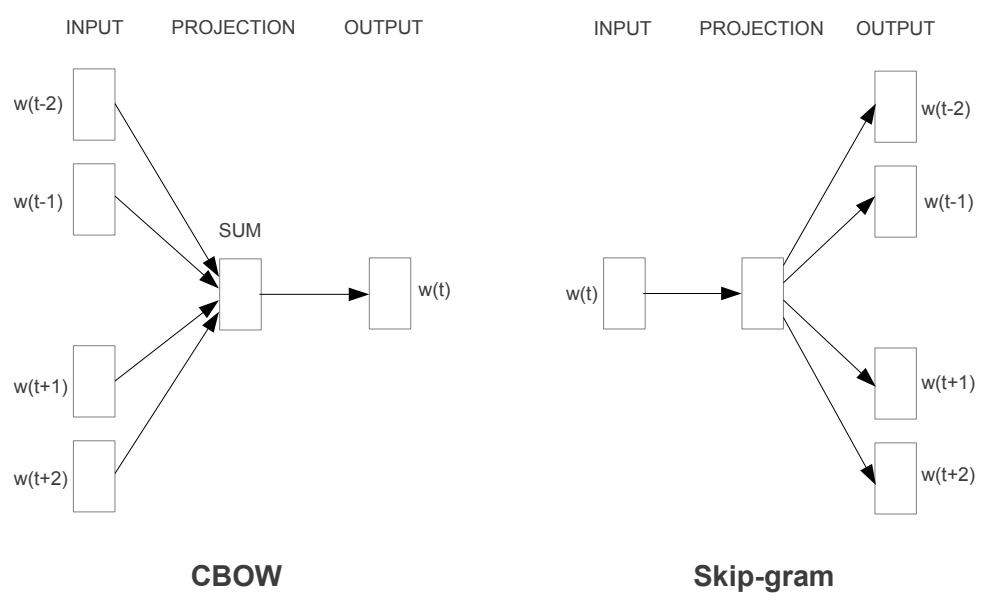
\includegraphics[width=\textwidth]{word2vec.png}
		\fonte{Taken from \citetexto[p.~5]{DBLP:journals/corr/abs-1301-3781}.}
	\end{minipage}
\end{figure}

After word2vec other algorithms emerged, such as \textbf{Global Vectors} (GloVe). \citetexto{Pennington2014} describes their work as "GloVe, is a new global log-bilinear regression model for the unsupervised learning of word representations that outperforms other models on word analogy, word similarity, and named entity recognition tasks.". GloVe is an approach that combines the global statistics of matrix factorization with the context based learning from word2vec.

\citetexto{Ling:2015:naacl} presents \textbf{Wang2vec} an extensions of the original word2vec models to improve the embeddings obtained for syntactically motivated tasks, by introducing changes that made the network aware of the relative positioning of context words.

Later on, \citetexto{bojanowski2016enriching} introduces \textbf{FastText}, which is another way to learn word representations by taking into account subword information. They incorporate character $n$-grams into the Skip-Gram model. By their evaluation the model outperforms baselines that do not take into account subword information.

% --------------------------

% The other family of word embedding model learns semantics by passing a window over the corpus line-by-line and learning to predict either the surroundings of a given word (Skip-gram model), or predict a word given its surroundings (continuous bag-of-words model). Note the bag-of-words problem is often shortened to “CBOW”.

% According to Mikolov et at., the authors of the word2vec paper, the two approaches differ slightly in performance:

% Skip-gram: works well with small amount of the training data, represents well even rare words or phrases.
% CBOW: several times faster to train than the skip-gram, slightly better accuracy for the frequent words.
% The authors of the GloVe paper note, however, that these context window-based methods suffer from the disadvantage of not learning from the global corpus statistics. As a result, repetition and large-scale patterns may not be learned as well with these models as they are with global matrix factorization. 

% Foram apresentados trabalhos relacionados ao tema abordado?
% Os trabalhos relacionados são relevantes para o tema investigado?
% Os trabalhos relacionados foram comparados com a pesquisa realizada?
% Os trabalhos relacionados são recentes?  Últimos 5 anos?
% Os trabalhos relacionados fizeram parte da discussão dos resultados da pesquisa realizada?



% Qual o problema abordado? hipotese?
% O que foi feito? Solução?
% Como foi realizada a avaliação?
% Comparar com o o meu trabalho - porque é relevante ao meu trabalho?


% G
\section{Related work}\label{chap:relatedwork}

In this section, will be presented works encountered while doing the bibliographic research. To find the state-of-the-art regarding word similarity, a search with Google Scholar\footnote{\url{https://scholar.google.com.br/}} and Semantic Scholar\footnote{\url{https://www.semanticscholar.org/}} was used. The terms used to find the related work in the field was "word similarity", "semantic similarity", "synonym", "Synonym extraction", "semantic embedding" and "morphological embedding". Also, some search through the Association for Computational Linguistics website\footnote{\url{https://aclweb.org/aclwiki/Similarity_(State_of_the_art)}} revealed some events regarding Semantic Textual Similarity, like the SemEval which were used to search for articles.

% TODO?: \subsection{trabalho denis}

\subsection{Comparing Semantic Relatedness between Word Pairs in Portuguese Using Wikipedia}

In this paper, \citetexto{GranadaSV14} presents a new dataset for evaluating Distributional Similarity Models in Portuguese. For this, they translated the word pairs from the well-know baseline for semantic relatedness evaluation in English called RG65 created by \citetexto{Rubenstein1965ContextualCO}. The original dataset contains judgements from 51 human subjects for 65 word pairs. To generate the PT65 they translated all the word-pairs and evaluated them with 50 human subjects. They compared the human scores with previous works and also performed a qualitative evaluation using Latent semantic analysis (LSA) models generated from Wikipedia articles. The correlation scores obtained were closer to the scores achieved by other works that targeted another language. With the experiement they observed that the semantic similarity can be transfered across languages, but for Portuguese, a manual evaluation had better results. 

With this, we intend to use the PT65 as a gold-standard for evaluating semantic similarity and relatedness between words with word embeddings models and the WordNet.

 

% Qual o problema abordado? hipotese?
% O que foi feito? Solução?
% Como foi realizada a avaliação?
% Comparar com o o meu trabalho - porque é relevante ao meu trabalho?


% G
\subsection{Dependency-Based Word Embeddings}

In this work \citetexto{Levy2014} presents a generalized skip-gram model with negative sampling introduced by \citetexto{Mikolov2013DistributedRO}, from a linear context of bag-of-words to arbitrary word contexts, specifically syntactic contexts. An interesting fact of this approach in comparison with the original work is that the concept of induced similarity represents a nature of \textit{cohyponym}. They also describe a way of performing an analysis of the representation learned in the vector space by exploring the contexts of specific words or a group of words.
They used the English Wikipedia as a corpus to train the embeddings. This corpus was tagged with parts-of-speech (POS) using the Stanford tagger. 

For the evaluation, they manually inspected the five most similar words to a hand-picked set of words. One remarkable example is the word "Hogwarts" that in the BoW model the most similar words are from the respective domain of Harry Potter and in the developed model it was a list of famous schools, that is, was able to capture the semantic type of the word.
The model was evaluated against the WordSim353 dataset from \citetexto{Finkelstein:2001:PSC:371920.372094}, which is a dataset regarding word similarity versus relatedness. They draw a precision-recall curve that describes the embeddings affinity, proving that the results obtained by the developed model were slightly better than the BoW model.



% Qual o problema abordado? hipotese?
% O que foi feito? Solução?
% Como foi realizada a avaliação?
% Comparar com o o meu trabalho - porque é relevante ao meu trabalho?

\subsection{Portuguese Word Embeddings: Evaluating on Word Analogies and Natural
Language Tasks}

\citetexto{Hartmann2017} present in this paper, an evaluation of different word embedding models trained on a large Portuguese corpus (Brazilian and European variants together) on syntactic and semantic analogies, POS tagging and sentence semantic similarity tasks.

They collected a large corpus from various sources, either in Brazilian or European Portuguese. With that they applied some preprocessing (Tokenization and normalization) in order to reduce the vocabulary size. Using the corpus as input, they trained some word embedding models using four different algorithms (Word2Vec, Wang2Vec, FastText and GloVe) with varying dimensions (50, 100, 300, 600 and 1000).

For the evaluation, first, they use the syntactic and semantic analogies provided by \citetexto{Rodrigues2016LXDSemVectorsDS}. Where the FastText model performed better for syntactic analogies while for semantic analogies GloVe had the best performance. Also, all CBOW models, except Wang2Vec, had very low results in semantic analogies.

For the POS tagging task evaluation, the Wang2Vec had the best results, and as seen, higher dimensions had better performance. The worst models in this task was GloVe and FastText. 

For the sentence semantic similarity task evaluation, they used the ASSIN dataset. With this they had Word2Vec CBOW model with 1000 dimensions as the best one for European Portuguese. And for Brazilian Portuguese the Wang2Vec Skip-Gram model with 1000 dimensions had the best scores.
In the end, they suggest that word analogies are not very suitable for evaluating word embeddings and task specific is probably a better approach.

We used they pre-trained word embedding models for comparison while evaluating our models under our specific task - word similarity on PT65.








% G
\subsection{ELMo and BERT}

\citetexto{Peters:2018} presents in this work, a general approach for learning context-dependent representations from bidirectional language models (biLMs). They called it Embeddings from Language Models (ELMo), and we can image it as a new kind of word embedding, that, instead of learning a word as a vector representation it has the intent to catch the context of a word as a vector representation, meaning that, it learns embeddings with the different nuances of a single word. Models like GloVe, Word2Vec, Wang2Vec, and FastText would generalize all the different nuances of a single word in a single word vector having the same representation. With the release of ELMo, it brought near state-of-the-art results in many downstream NLP tasks,  including question answering, textual entailment, and sentiment analysis.

ELMo induced the current state-of-the-art technique called BERT, which stands for Bidirectional Encoder Representations from Transformers.  
BERT, a work by \citetexto{devlin2018bert}, is a method of pre-training language representations. It outperforms previous methods because it is the first unsupervised, deeply bidirectional system for pre-training NLP. It uses attention transformers instead of bidirectional RNNs to encode context.

As these works represent the state-of-the-art evolution from the first word embeddings and allow pre-trained models to be used for general purpose NLP tasks, we intend to explore how these language models behave for word-level tasks such as word similarity. 


\subsection{Distributional and Knowledge-Based Approaches for Computing Portuguese Word Similarity}

In this work \citetexto{gonccalo2018distributional}, presents several approaches for computing word similarity in Portuguese where they make an extensive comparison between these different approaches, which includes word embeddings and lexical knowledge bases. The comparison aims, for each approach, the effectiveness in this particular task as well as the quality and coverage of words. For the evaluation, they do a qualitative analysis of the results based on four datasets that have been recently adapted to Portuguese, PT65, SimLex-999, WordSim-353, and RareWords.
The results of this work indicate that distributional models capture relatedness better than lexical knowledge bases which seems to be better suited genuine similarity.


\subsection{Discussions}

Based on these works, we evaluated the WordNet against the word embedding approach regarding the identification of word similarity using several word embedding algorithms. 
We used the pre-trained word embedding models presented by \citetexto{Hartmann2017} for comparison while evaluating our models under our specific task of word similarity identification.
Moreover, we adapt the work of \citetexto{Levy2014} to generate a word embedding with syntactic contexts from a Brazilian Portuguese corpus, to check if the results were, similar or not regarding other models, but instead of using the WordSim353 which is for English, we used another dataset that can be considered a gold standard for our target language.
Because of the results presented by \citetexto{GranadaSV14}, we ended up using the PT65 as a gold-standard for evaluating semantic similarity and relatedness between words with word embedding models and the WordNet. 

Regarding the work from \citetexto{gonccalo2018distributional}, they didn't evaluate different dimension sizes for the word embedding models, also they didn't compare results with the DEPS word embeddings that includes syntactic knowledge, so in our work we intend to do this evaluation and also compare results with our own generated word embeddings, instead of comparing only the NILC available ones.


Also, regarding the works from \citetexto{Peters:2018} and \citetexto{devlin2018bert}, as they represent the state-of-the-art evolution from the first word embedding models and allow pre-trained models to be used for general purpose NLP tasks, we intend to explore how these language models behave for word-level tasks such as word similarity.

% \subsection{A study on similarity and relatedness using distributional and WordNet-based approaches}

In this paper, \citetexto{Agirre2009} compares the two main categories of techniques used to measure semantic similarity. Using graph-based algorithms to Word-Net and distributional similarities collected from a 1.6 Terabyte Web corpus. A joint of the two techniques are also explored.

For the graph-based algorithm they represent WordNet version 3.0 as a graph, where the relations among synsets are undirected edges, and for this graph, the PageRank is computed for each of the words in the corpus producing a probability distribution over synsets. Then, this is encoded as vectors by computing the cosine between them. In this word two WordNet versions were used, the WordNet 3.0 and the Multilingual Central Repository (MCR) aiming to link words between multiple WordNet languages. For cross-linguality, they exchange each non-English word in the dataset with its 5 best translations into English and then create the vector with the calculated similarities.

For the distributional approach of calculating similarities between words the explore the use of a vector space model using three variations as bag-of-words, context-window and syntactic-dependency over a corpus of four billion documents crawled from the web in August 2008.

They evaluate all the approaches over two standard datasets (RG65 and WordSim353) and also test a combination of both approaches (WordNet and Distributional) by training an SVM classifier to select the best result of the tree distributional variations for each pair. Thus, achieving state-of-the-art distributional and WordNet-based similarity measures over this datasets.

% \subsection{Morphological Word Embeddings}

% % TODO: Falta o como foi feito técnicamente
% % TODO: breve descrição do porque é relevante para o meu trabalho

% In this work, \citetexto{Cotterell2015MorphologicalW} propose a new model, Morph-LBL, for the semi-supervised induction of morphologically guided embedding. The raw text was annotated with morphological data with the intent to create word embeddings that preserve the morphological relations of the words. The motivation for doing this is the hypothesis that languages with a high morpheme per word ratio would have improved results if we take into account the morphological information of the words.

% They extend the log-bilinear model (LBL) by training with a corpus annotated with morphological tags. A very interesting point is that only a part of the corpus was annotated with the tags, only to initially guide the embeddings with the intention that they maintain their morphological characteristics during the rest of the training.
% Qualitative evaluation was performed by attempting to determine if a word close in the vector space model is also morphological close to another and in fact, they were.
% They also introduced a new metric for quantitative evaluation of the model, named MorphoDist, that they used to compare with other models, and the Morph-LBL surpassed the original Skip-Gram model and Log-Bilinear Model.

% \subsection{A Minimally Supervised Approach for Synonym Extraction with Word Embeddings}

% % TODO: Falta o como foi feito técnicamente
% % TODO: breve descrição do porque é relevante para o meu trabalho

% In this work, \citetexto{Leeuwenberga2016} investigates the use of word embeddings for automatic extraction of synonyms from a corpus. Their initial motivation came from machine translation evaluation where hypothesis translations are automatically compared with reference translations using a system that do this kind of evaluation named Meteor. Meteor is composed of four modules and one of them is synonym matching that currently uses WordNet for such a task. One problem with WordNet is that it is not available to all languages. So, the idea here is to use Word Embeddings a synonym matcher and in that case, it could be available to multiple languages as the training of word embeddings is unsupervised.
% They trained the word embeddings using three different approaches, CBoW, SG, and GloVe over English and German.  Also, they used a part-of-speech (POS) tagger to improve the synonym extraction. For evaluation, synonyms were obtained from WordNet 3.0 for English and GermaNet 10.0 for German.
% They excluded the results for the GloVe vectors, as they showed lower precision than SG and CBOW, and they did not use them in further experiments.
% From these experiments, they conclude that POS tags can help to slightly improve synonym extraction.

% ------------------------------------------------------------------
% \subsection{A Minimally Supervised Approach for Synonym Extraction with Word Embeddings}

% They use word embeddings aiming to be extensible to various languages. 

% They came up with a new similarity metric, relative cosine similarity, and show that this metric improves the extraction of synonyms from raw text. They also employ the extracted synonyms in the synonymy module of Meteor and use human evaluation to judge the quality of synonyms extracted.

% . Approaches like Meteor (Denkowski and Lavie, 2014; Banerjee and Lavie, 2005) computes an alignment between the hypothesis and reference to
% determine to what extent they convey the same meaning. Finding possible matches is done by means of four modules. One of them is synonym matching, that uses a synonym database resource to match words which may not be string identical. The module uses synonyms from the lexical database WordNet (Miller, 1995) and for this reason, not available for all languages. 
% Manual construction of lexical resources such as WordNet is time-consuming and expensive and needs to be done for each different language.

% Different experiments over the use of word embedding were carried out. First, they analyze the effect of contextual window size, the number of dimensions, and the type of word vectors on the precision of extraction, for English and German. Secondly, they look closely at the word categories that are (cosine) similar in the vector space. Then, they look at cosine similarity and introduce relative cosine similarity. Lastly, they examine the overlap of the most similar words in different vector spaces.

% They trained the word embeddings using three different approaches, CBoW, SG, and Global Vectors (GloVe) (Pennington et al., 2014) using different parameters with a 150 million word subset of the NewsCrawl corpus for English and German. Lowercasing, tokenization, and digit conflation were applied as preprocessing for both languages. Also, they used a part-of-speech (POS) tagger to improve the synonym extraction. For evaluation, synonyms were obtained from WordNet 3.0 for English and GermaNet 10.0 for German.

% They excluded the results for the GloVe vectors, as they showed lower precision than SG and CBOW, and they did not use them in further experiments. The general trends of the GloVe vectors were that they had higher precision for larger window sizes. The vectors with highest precision of 0.067 for English were of dimension 300, with a window size of 32. For German, the highest precision was 0.055, and the vectors were of dimension 1200, with a window size of 32 as well.

% For evaluation, they use the synonyms from WordNet 3.0 for English, and GermaNet 10.0 for German. In both WordNet and GermaNet words carry a corresponding part-of-speech. InWordNet these are nouns, verbs, adjectives, and adverbs. In GermaNet, synonyms are given for nouns, verbs, and adjectives. Because a given word’s part of speech is unknown here, we consider the synonyms of each word to be those of all the parts of speech it can potentially have inWordNet or GermaNet.
% 3.2.

% They develop a different measure to calculate similarity relative to the top n most similar words between word wi and wj as:

% \begin{equation}
%   rcs_n(w_i,w_j) = \frac{cosine_similarity(w_i,w_j)}{
%   \sum_{w_c\epsilon TOP_n} cosine_similarity(w_i,w_c)
%   }
% \end{equation}

% In order to separate some word senses we preprocessed both the English and German corpora from the previous chapter with the Stanford POS tagger (Toutanova et al., 2003), using the fastest tag-models. To compare using the simplified POS tags with the previous approaches we also calculated precision, recall and f-measure on Stest. Compared to the baseline of looking only at the most-similar word,we found that recall in English increased from 3\% to 4\%, precision did not change (11\%), and f-measure from 5\% to 6\%. Notably, German precision increased with 8\% to 12\%, recall from 5\% to 7\%, and f-measure from 6\% to 9\%. From these experiments we conclude that POS tags can help to improve synonym extraction in three ways. Firstly, they can separate some of the word senses, however this effect is minor. Secondly, they can filter words that are not grammatically similar enough, such as plurals. And thirdly, they can exclude synonyms in categories for which there no, or very few, synonyms, such as names.

% \subsection{UMBC EBIQUITY-CORE: Semantic Textual Similarity Systems}

% In this paper, \citetexto{Han2013} presents a hybrid word similarity model that was used in semantic text similarity systems developep for the *SEM 2013 STS shared task were they achieved first place of the 89 submitted runs.

% Their model was originally developed for the Graph of Relations project which maps informal queries with English words and phrases for an RDF linked data collection into a SPARQL query. The model combines LSA word similarity and WordNet knowledge.



% As this work, aims to compare techniques of word similarity based on two approaches,  lexical bases and distributional, we did some evaluation on 
% use a common portuguese dataset for evaluation called PT65 and 
% In order to be able to generate the word embeddings using multiple algorithms, it is required a corpus. For this, we got a portuguese Wikipedia dump and did some pre-processing to generate a corpus suitable for the given task.
% This work aims to compare techniques based on lexical bases with the distributional based ones.

% - Explore the existing techniques regarding word similarity, using a distributional approach called word embeddings, adapting existing works to Brazilian Portuguese.
% - Compare the word embeddings approach to other techniques that are solely based on a lexical database such as WordNet.
% - Adapt existing studies regarding the addition of syntactic context in the training process of word embeddings to a Brazilian Portuguese corpus, to check if the results will be, similar or not. 
% - Evaluate the different techniques over a common \textit{dataset}.

% \subsubsection{WordSimilarity-353 Test Collection}
% The WordSimilarity-353 is a test collection for measuring word similarity developed by \citetexto{Finkelstein:2001:PSC:371920.372094}. This dataset contains two sets of English word pairs along with human-assigned similarity judgements.
% http://www.cs.technion.ac.il/~gabr/resources/data/wordsim353/
% \subsubsection{ENSEPRO Word Similarity}
% Aiming to prove an improvement in the accuracy of information extraction systems, a specific dataset will be assembled using the questions and answers of short sentences used in the ENSEPRO system. This system evaluation was made using the dataset for the challenge Question Answering over Linked Data (QALD-7) of 2017, which also had the addition of the Portuguese language. For each sentence of the Portuguese questions of this dataset, we will assemble a new dataset with only the keywords necessary to carry out queries via the ENSEPRO search engine. A pair of this keyword must be generated with the one that is currently in the linked data. For words that the system currently cannot find answers due to lack of a word in the expansion of related terms, it will be investigated manually which would be the word that should be found and added to the dataset. Also, the dataset will include the syntactic information for each keyword.



\section{Methods and materials}\label{chap:methodsandmaterials}

This chapter will present a description of what and how this work was done, as well as the tools and methods used. First ~\autoref{chap:methodsandmaterials:architecture} presents an overview of the architecture and how the proposed experiment was realized. Then, the ~\autoref{chap:methodsandmaterials:dataset} presents the dataset used in the evaluation process. After that we start with a detailed explanation of the Corpus generation in ~\autoref{chap:methodsandmaterials:corpus}.
% Finally in the ~\autoref{chap:methodsandmaterials:evaluation}, is shown how the evaluation was performed.

\subsection{Architecture overview}\label{chap:methodsandmaterials:architecture}

The proposed work basically consists of comparing different word similarity techniques. Therefore, ~\autoref{fig:arq} defines an overview of the architecture with the intention of comparing several techniques using different algorithms and testing them with a common dataset.

\begin{figure}[h]
	\caption{Proposed architecture}
	\label{fig:arq}
	\centering%
	\begin{minipage}{.8\textwidth}
		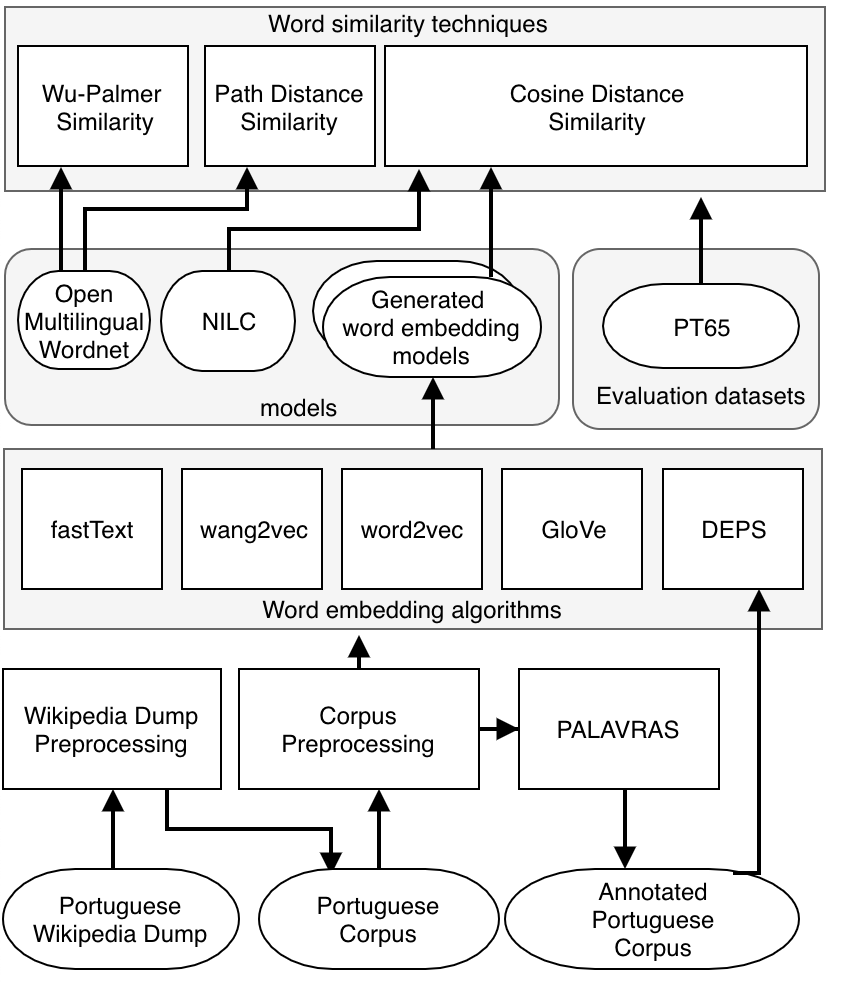
\includegraphics[width=\textwidth]{arq.png}
		\fonte{Made by the author.}
	\end{minipage}
\end{figure}


In this work we compared techniques based on the two main approaches to word similarity, the knowledge-based and the distributional-based. 

Regarding the knowledge-based approach we utilized a lexical base, in this case, \textbf{Open Multilingual Wordnet} (OMW) wore used with \textbf{Path Distance} and \textbf{Wu-Palmer} similarity techniques. It was decided to use OMW due to its ease of use through the \textbf{Natural Language Toolkit} (NLTK) library available for the \textbf{Python version 3.6} programming language as well as the availability of the Portuguese language for querying the synsets.

For the distributional approach we \textbf{generated word embedding models} with a corpus obtained from the \textbf{brazilian portuguese Wikipedia dump} of articles. The word embeddings wore generated using several diferent model implementations for learning word representations. In this case, \textbf{FastText}, \textbf{Wang2vec}, \textbf{Word2vec} and \textbf{GloVe}. Also, we compare our word embedding models with a set of pre-trained models available by \textbf{Núcleo Interinstitucional de Linguística Computacional} (NILC) in all different implementations (FastText, Wang2vec, Word2vec and GloVe). One thing to note is that, the metric used for the comparison of similarity between one word and another for all word embedding models was the \textbf{cosine distance}. The \textbf{CBOW} and \textbf{Skip-gram} were used for the models that has this option.

We also generated one more model in order to take into account the syntactic tree information of the sentences from the Portuguese corpus using the algorithm implementation by \citetext{Levy2014} wich generates the \textbf{DEPS} (Word2vecf) model. In order to do this, we used the \textbf{PALAVRAS syntactic parser} to annotate the corpus with syntactic information.

In the end we do a quantitative evaluation of all models and techniques using the \textbf{PT65} dataset, which consists in a pair of words and a similarity value given by persons.

All the experiments were done using the \textit{Semantics} computer (Intel(R) Xeon(R) CPU E5-2620 v4 @ 2.10GHz with 32 cores and 128GB of RAM) granted by the \textit{Unisinos Programa de Pós-graduação em Computação Aplicada} (PPGCA) by running \textbf{Docker} containers.


\subsection{PT65 Dataset}\label{chap:methodsandmaterials:dataset}

This dataset is composed by 65 word pairs, initialy generated by \citetexto{Rubenstein1965ContextualCO} on the name of \textit{RG65}. This word pairs wore translated to portuguese by \citetexto{GranadaSV14} and evaluated with 50 persons. 

The initial idea was to use the WordSimilarity-353 Test Collection developed by \citetexto{Finkelstein:2001:PSC:371920.372094} which consists of two sets of English word pairs along with human-assigned similarity judgements. But we would have to translate to portuguese and then the human-assigned similarity judgements would not fit entirelly regarding the semantic changes involved in the translation proccess. So the PT65 dataset was used in the evaluation process.

\subsection{Corpus generation}\label{chap:methodsandmaterials:corpus}

In this section, I will present the process involved in generating a corpus that can be used on NLP tasks from a Wikipedia dump. I’ve used this process to generate the Word Embeddings for evaluation in this thesis. While I focus on the Portuguese language, you could easily do the same thing for the other available languages in Wikipedia.

\subsubsection{Getting the Wikipedia PT-BR dump}

First, we downloaded the latest Portuguese Wikipedia articles dump\footnote{\url{https://dumps.wikimedia.org/ptwiki/latest/ptwiki-latest-pages-articles-multistream.xml.bz2}}. The file is a big, compressed XML file that contains all articles in the wiki text format, just like markdown but with some special tokens that deal with some specific Wikipedia features. For example: "\textit{[[Imagem:Starsinthesky.jpg|thumb|[[Estrela|Formação estrelar]] na [[Grande Nuvem de Magalhães]], uma [[galáxia irregular]].]]}"

% \begin{lstlisting}
%     @[[Imagem:Starsinthesky.jpg|thumb|[[Estrela|Formação estrelar]] na [[Grande Nuvem de Magalhães]], uma [[galáxia irregular]].]]@
% \end{lstlisting}

You can find more detailed information about the dump formats and different languages in their website\footnote{\url{https://en.wikipedia.org/wiki/Wikipedia:Database_download}}.

\subsubsection{Preprocessing with Wikiextractor}

As described in the previous step, the format of the dump is not suitable for most of NLP tasks. That’s why we need to parse the wiki text format to raw text. In order to do this, we have a few options. We could use the python \textbf{gensim.corpora.WikiCorpus} class but its tokenizer is not so good for Portuguese (In our case we need to have words separated by ‘-’ like ‘guarda-chuva’ which is very common in Portuguese). So, we ended up using the \textbf{wikiextractor} project that just reads the XML file and outputs all the documents in parsed text. We chose to cleanup and tokenize the corpus in a later stage. So, we just cloned the repository and executed the \textbf{wikiextractor}.

% \begin{lstlisting}[language=sh]
% git clone https://github.com/attardi/wikiextractor.git
% cd ./wikiextractor
% python ./WikiExtractor.py --no-templates -o ../data/ptwiki-articles-text/ -b 10M -c ../data/ptwiki-latest-pages-articles-multistream.xml.bz2
% cd ..
% \end{lstlisting}

Wikipedia has a concept of Templates, which consists of using other documents inside of a given one. For the objective of this corpus, it is not desired that the tool expands these templates, because it will just add duplicated sentences to the content. So, it is really important to use the \textit{–no-templates} flag.
This tool generated multiple compressed 10MB files of wiki articles sentences as seen in ~\autoref{fig:wikiextractor}.

\begin{figure}[h]
	\caption{WikiExtractor output sample.}
	\label{fig:wikiextractor}
	\centering%
	\begin{minipage}{.9\textwidth}
		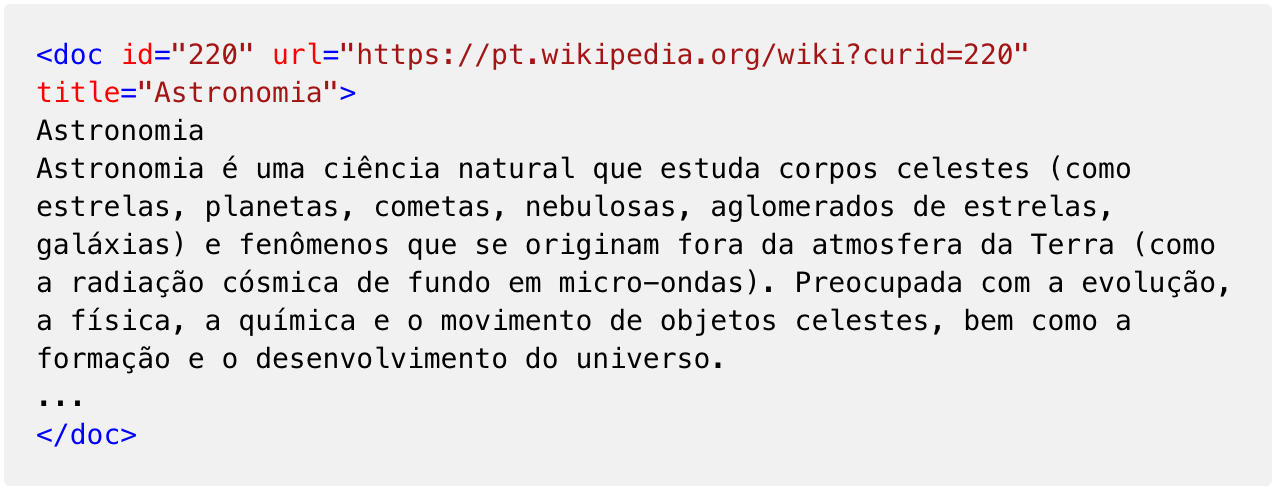
\includegraphics[width=\textwidth]{wikiextractor.png}
		\fonte{Made by the author.}
	\end{minipage}
\end{figure}



% \begin{lstlisting}[language=XML]
% <doc id="220" url="https://pt.wikipedia.org/wiki?curid=220" title="Astronomia">
% Astronomia 
% @Astronomia é uma ciência natural que estuda corpos celestes (como estrelas, planetas, cometas, nebulosas, aglomerados de estrelas, galáxias) e fenômenos que se originam fora da atmosfera da Terra (como a radiação cósmica de fundo em micro-ondas). Preocupada com a evolução, a física, a química e o movimento de objetos celestes, bem como a formação e o desenvolvimento do universo.@
% ...
% </doc>
% \end{lstlisting}

It is also possible to save this as only one text file just by changing the tool arguments.
At the time of writing, there were 1,000,400 documents in the ptwiki-dump.

\subsubsection{Custom preprocessing}

In order to cleanup the sentences for generating the Word embedding models we did some custom pre-processing\footnote{\url{https://github.com/eberlitz/pt-br-word-embeddings/blob/master/scripts/preprocess.py}} based on \citetexto{Hartmann2017} preprocessing scripts. Some changes were made to do the some cleaning as follows:

\begin{itemize}
    \item Breaks an entire document into multiple sentences using the 
    \textbf{nltk.data.load ('tokenizers/punkt/portuguese.pickle')}. (Natural Language Toolkit - NLTK is a leading platform for building Python programs to work with human language data, and it has a sentence segmentation tool called \textbf{punkt}.)
    \item Does not change the current letter case. (Later I'll use a Syntactic parser that has better accuracy if I maintain this)
    \item Remove sentences with less than 4 tokens (as it does not add meaningful value to the corpus we can remove very short sentences).
    \item Allow abbreviations, like 'Dr.'.
    \item Keep words with '-', like 'guarda-chuva' (which means umbrella in English).
    \item All emails are mapped to EMAIL token.
    \item All numbers are mapped to 0 token.
    \item All URLs are mapped to URL token.
    \item Different quotes are standardized.
    \item Different kinds of hyphenation are standardized.
    \item HTML strings are removed.
    \item All text between brackets is removed.
\end{itemize}

With this, we ended up with the final 1.6GB PT-BR corpus file which contains 9.896.520 sentences, 251.193.592 tokens and 3.137.040 unique tokens.

% --------------------------------------------------------

\subsection{PALAVRAS annotated corpus generation}\label{chap:methodsandmaterials:palavras}

To annotate all sentences of the corpus with syntactic tags, we used the software PALAVRAS developed by \citetexto{bick2000palavras}, which is an automatic parser for Portuguese.

First, we tried to use the parser with multiple sentence files of 1MB. However, the parser was taking too much time to execute and sometimes errors occurred. So we wrote a Python script that sends sentences in batches to the PALAVRAS parser and saves the results. Also, we have used parallel computing doing this process times the number of cores on the machine. Although, we first run this on a i5 2.4GHz computer with 4 cores, achieving an average speed of 16 sentences per second, which means that for all 9896520 sentences it would take 7 days to complete. We have tried other techniques attempting to increase the speed, but the bottleneck was indeed in the parser tool. 

With this problem at hand, \textit{UNISINOS Programa de Pós-graduação em Computação Aplicada} (PPGCA) granted us access to the \textit{Semantics} computer (Intel(R) Xeon(R) CPU E5-2620 v4 @ 2.10GHz with 32 cores and 128GB of RAM). With 32 cores the parsing step should be concluded in 24 hours.

One more problem that we had is that the PALAVRAS could not parse some of the sentences. Since we were running the parser in batches, this means that if one sentence failed, we lost all the parsed sentences in the batch. Also, as this process would take too long, we had to implement some way to continue the process if some fatal error occurred. With this in mind, we converted the sentences file to an SQLite table with three columns (id, text and parsed text). With this whenever we start the parsing process, we can continue from where it stopped.

With this solution implemented, we created a docker image and started running in the Semantics machine. The overall process took 38 hours. 24 hours to process 8916000 sentences using batches of 30, and 14 hours to process the remaining ones without sending in batches. Resulting in a 15GB corpus file.

% --------------------------------------------------------

\subsection{Common Word Embeddings generation}\label{chap:methodsandmaterials:wegeneration}

In order to have a base for comparison, we generated all models that were used by \citetexto{Hartmann2017}. In this case, FastText, Wang2vec, Word2vec and GloVe using different dimensions values as 50, 100, 300, 600 and 1000. \cite{bojanowski2016enriching, Ling:2015:naacl, Mikolov2013DistributedRO, Pennington2014}. Also the CBOW and Skip-gram were used for the models that has this option.

For this, we downloaded all those model generation tools from GitHub, compiled into a docker image, and use as input our corpus text file. We only created some script to run this several times with different dimension sizes as it took several hours to complete.

% --------------------------------------------------------

\subsection{DEPS Word Embedding generation}\label{chap:methodsandmaterials:depsgeneration}

In order to generate the DEPS (dependency-based syntactic contexts) word embedding model proposed by \citetexto{Levy2014}, we got the source code called \textit{word2vecf} from their website. The input required by this model is three files, a word and context vocabulary, and a contexts file. 

The vocabulary files are just a list of words or contexts with the total number of occurrences. The contexts file is a multiline context per word, where one word can have multiple contexts. In the form of "<\textit{word}> <\textit{dependency-relation}>\_<\textit{referred-word}>".

In order to generate this file from our corpus we got the annotated output from the PALAVRAS parser and extracted the syntactic tags. This process is shown by in ~\autoref{fig:deps-context}.

\begin{figure}[h]
	\caption{DEPS contexts generation from parsed sentence. Left: Sample output from the PALAVRAS parser for the sentence "A astronomia é uma das mais antigas ciências.". Right: Sample of our generated contexts file for an annotated sentence.}
	\label{fig:deps-context}
	\centering%
	\begin{minipage}{.95\textwidth}
		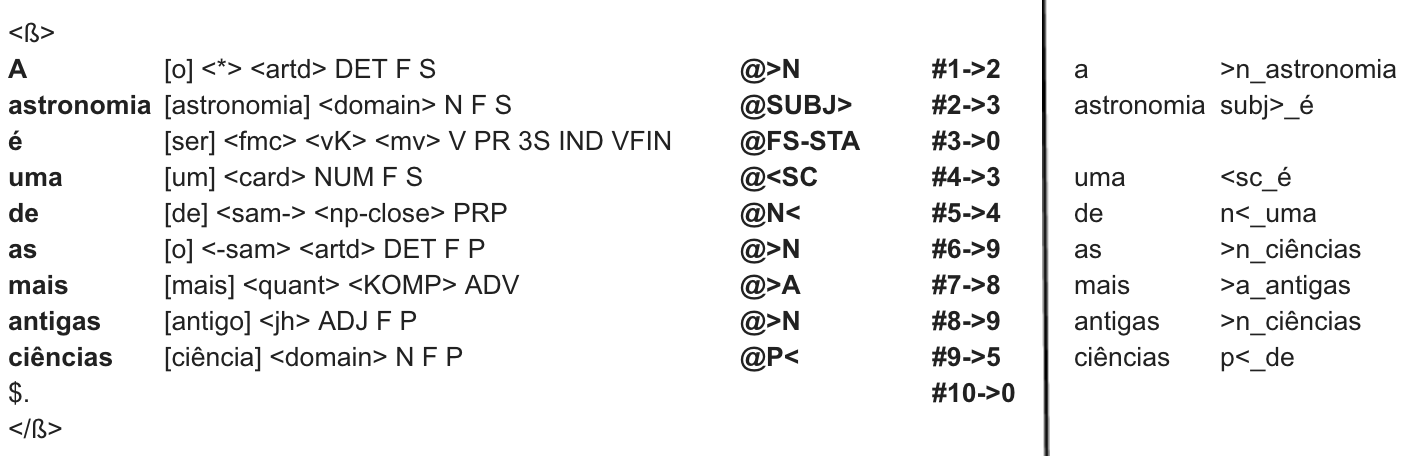
\includegraphics[width=\textwidth]{deps-context.png}
		\fonte{Made by the author.}
	\end{minipage}
\end{figure}

The generation of this three files was not trivial and the implemented code to do so had to use a map-reduce approach in order to use all computation resources available. It took 14 hours to process all 9896000 parsed sentences with an average speed of 196.2 sentences per second.

After we had the input files, we just run the \textit{word2vecf} tool which took some hours to complete. We generated models with different dimensions values as 50, 100, 300, 600 and 1000.








% CÓDIGO: https://levyomer.wordpress.com/2014/04/25/dependency-based-word-embeddings/
% DATASET: http://www.cs.technion.ac.il/~gabr/resources/data/wordsim353/

% resources:
% - Open Multilingual Wordnet
% - NILC Pre-trained word embeddings models
% Corpus:
%  - Pegar com o allan o corpus portugues
%  - Anotar o corpus com o PALAVRAS syntactic parser
% quantitative evaluation datasets:
%  - WordSim353 manual translation to portuguese
%  - ENSEPRO word similarity (vou criar em conjunto com o denis, preciso definir formato e como, usando as perguntas do QALD)
% Algoritmo:
%  - Usar o código fonte do DEPS
% tools:
%  - Palavras
%  - Python NLTK, word2vec, word2vecf, 













% \begin{itemize}
%     \item Explore the existing techniques regarding word similarity, using a distributional approach called word embeddings, adapting existing works to Brazilian Portuguese.
%     \item Compare the word embeddings approach to other techniques that are solely based on a lexical database such as WordNet.
%     \item Adapt existing studies regarding the addition of syntactic context in the training process of word embeddings to a Brazilian Portuguese corpus, to check if the results will be, similar or not. 
%     \item Evaluate the different techniques over a common \textit{dataset} related to \citetexto{denis2018} work.
% \end{itemize}

% This thesis is structured as follows. The \autoref{chap:background} presents the general concepts and techniques used in this work. In \autoref{chap:relatedwork} are described and analyzed the works related to the research area of this work. The \autoref{chap:methodsandmaterials} presents the proposed model, as well as the form of the experiment and the necessary tools. The \autoref{chap:results} presents the preliminary results obtained in the case study experiment. Finally, \autoref{chap:conclusions} summarizes the thesis findings, contributions, and discusses.





% Descrever um cenário em que o projeto se faz necessário (Extração de informação em ontologias utilizando Linguagem Natural - Talvez citar o uso de queries que utilizem triplas RDF) e ajuda a resolver o problema. Após descrito citar como exemplo o trabalho do denis e detalhar o cenário dele.

% - Cenário do denis: Recebe uma pergunta; Realiza um parse, extraindo palavras relevantes e seu contexto sintático; Realiza a geração de combinações diferentes de possíveis tuplas RDF de pesquisa; Algumas dessas pesquisas não se encontra a resposta, porém se uma destes elementos da tupla fosse substituído por um outro sinônimo ele iria encontrar a resposta. Portanto é usado o WordNet BR para procurar por sinônimos, porém ainda assim, nem sempre se tem a palavra cadastrada no WordNet.

% Descrever a arquitetura do modelo proposto.

% - Usar o NLTK python e procurar por sinônimos de uma dada palavra no OpenWordNet-PT ( supõe-se que algumas vezes não será encontrado nada )
% - Usar diferentes tipos de word embedding (BoW, SG, GloVe)
% - [TCC2]Treinar word embeddings sobre um corpus (pegar com o allan) utilizando o contexto gerado pelo POS Tagger da unisinos (Aonde consigo??)
% - [TCC2]Algum outro algoritmo se houver necessidade
% - Testar cada abordagem com o dataset do denis




% OpenWordNet-PT. \cite{coling2012}.


\section{Results}\label{chap:results}


We separate the evaluation in three steps. In \autoref{chap:results:wn} we do a quantitative evaluating of the Open Multilingual WordNet. In \autoref{chap:results:we} we do the same evaluation but with the word embeddings models. At last, we do a qualitative evaluation regarding the DEPS model in \autoref{chap:results:qualitative}

% For the evaluation, we propose to do qualitative measure based on a manual inspection of the most similar words to a hand picked set of words and see if they are in fact similar or not to the other words regarding similarity, relatedness and also the syntactic similarity.
% Also a quantitative analyses is proposed by using the WordSim353 dataset from \citetexto{Finkelstein:2001:PSC:371920.372094}, which is a dataset regarding word similarity versus relatedness. As all the pairs in this dataset are in English, they will be manually translated to Portuguese to be able to compare the results with all the techniques.
% To better visualize the performance of each technique the precision-recall curve draws will be used to describes the embeddings affinity.
% Another quantitative analysis will be done to see if the recall increase using the ENSEPRO dataset. If it increases it will improve the quality of the ENSEPRO system. 


\subsection{Open Multilingual WordNet evaluation}\label{chap:results:wn}

In order to do a quantitative evaluation of the knowledge-based approach for word similarity. We used the Open Multilingual Wordnet (OMW) from \citetexto{Bond2013LinkingAE} and loaded it with the Natural Language Toolkit (NLTK) library. We then calculated the similarity between the pair of words from the PT65 dataset using two algorithms, Path Distance and Wu-Palmer. With this we calculated the Pearson’s Correlation ($\rho$) for each of the techniques.

\autoref{tab:worneteval} shows the results, and as we can see, the Path Distance algorithm gave a relative high score, but as stated by \citetexto[p.~297]{Jurafsky:2009:SLP:1214993} we indeed have out of vocabulary words, in this case 15.38\% of the words.


\begin{table}[h]
    \caption{OMW evaluation on PT65.\textbf{$\rho1$} is the Pearson’s Correlation considering only the words in vocabulary; \textbf{$\rho2$} is the Pearson’s Correlation considering all the words, given a similarity value of zero for words out of vocabulary. }
    \label{tab:worneteval}
    \centering%
    \begin{minipage}{.8\textwidth}
    \begin{tabular}{@{}lllll@{}}
    \cmidrule(r){1-5}
    \textbf{Algorithms} & \textbf{$\rho1$} & \textbf{$\rho2$}         & \textbf{Out of vocabulary ratio} \\ 
    \cmidrule(r){1-4}
    Path Distance & \textbf{0.76} & 0.67   & 15.38                   \\
    Wu-Palmer     & 0.62    & 0.51         & 15.38                   \\ \cmidrule(r){1-4}
    \end{tabular}
    \fonte{Made by the author.}
    \end{minipage}
\end{table}





% OWM, path, 0.7629920696961829, 1.2781571648596962e-11, 0.638215045981246, 1.5911706121638655e-07, 15.384615384615385
% OWM, wup, 0.6224196059044503, 3.9086124786740125e-07, 0.5993354805660435, 1.3336702025718145e-06, 15.384615384615385
% OWM, path, 0.6755297783884997, 6.699886211511832e-10, 0.537623366025965, 3.8731549459381025e-06, 13.333333333333334
% OWM, wup, 0.5130904887818083, 1.2406652833034867e-05, 0.5101121482658979, 1.4203800232966779e-05, 13.333333333333334




\subsection{Word embeddings Evaluation}\label{chap:results:we}

To do a quantitative evaluation of the distributional approach for word similarity we did the same experiement as the WordNet evaluation but with our word embeddings models.
We loaded the PT65 dataset and for each pair of word we compared the expected result with the Cosine similarity given by the model. With this we calculated the Pearson’s Correlation ($\rho$).

\autoref{tab:evaluation:we} shows the results for all the 40 generated models. There was no out of vocabulary words in this approach which in comparison with the wordnet approach is better, just like mentioned by \citetexto{Agirre2009} we can use word embeddings to cover out-of-vocabulary words. Also we can see that the better word embedding model for this task is the FastText Skip-Gram. And in all of them Skip-gram was slighty better than the others. And in overall the models with 300-600 dimensions got higher values. We can also note that the DEPS model have a very poor performance in this particular task, maybe because the dataset do not differentiate between relatedness and similarity.

We also repeated the same experiement with the pre-trained models by \citetexto{Hartmann2017} from Núcleo Interinstitucional de Linguística Computacional (NILC).


\begin{table}[]
    \caption{Word embeddings evaluation on PT65. \textbf{$\rho(ours)$} is the Pearson’s Correlation value from our trained models. \textbf{$\rho(nilc)$} is the Pearson’s Correlation values from the NILC pre-trained models.}
    \label{tab:evaluation:we}
    \centering%
    \begin{minipage}{.65\textwidth}
    \begin{tabular}{@{}lllll@{}}
    \cmidrule(r){1-5}
    \textbf{Embedding Models} &      & \textbf{Size} & \textbf{$\rho(ours)$} & \textbf{$\rho(nilc)$} \\ \cmidrule(r){1-5}
    FastText            & CBOW          & 50   & 0.67             & 0.63            \\
                        &               & 100  & 0.72             & 0.67            \\
                        &               & 300  & \textbf{0.75}    & 0.73            \\
                        &               & 600  & 0.73             & 0.74            \\
                        &               & 1000 & 0.71             & 0.74            \\ \cmidrule(lr){2-5}
                        & Skip-Gram     & 50   & 0.74             & 0.64            \\
                        &               & 100  & \textbf{0.77}    & 0.73            \\
                        &               & 300  & \textbf{0.79}    & \textbf{0.78}   \\
                        &               & 600  & \textbf{0.77}    & \textbf{0.76}   \\
                        &               & 1000 & 0.72             & 0.74            \\ \cmidrule(r){1-5}
    Wang2vec            & CBOW          & 50   & 0.57             & 0.59            \\
                        &               & 100  & 0.61             & 0.69            \\
                        &               & 300  & 0.69             & 0.74            \\
                        &               & 600  & 0.69             & 0.66            \\
                        &               & 1000 & 0.68             & 0.65            \\ \cmidrule(lr){2-5}
                        & Skip-Gram     & 50   & 0.65             & 0.60            \\
                        &               & 100  & \textbf{0.74}    & 0.70            \\
                        &               & 300  & \textbf{0.75}    & \textbf{0.77}   \\
                        &               & 600  & 0.72             & \textbf{0.76}   \\
                        &               & 1000 & 0.69             & x.xx            \\ \cmidrule(r){1-5}
    Word2vec            & CBOW          & 50   & 0.58             & 0.34            \\
                        &               & 100  & 0.63             & 0.43            \\
                        &               & 300  & 0.68             & 0.58            \\
                        &               & 600  & 0.69             & 0.62            \\
                        &               & 1000 & 0.68             & 0.61            \\ \cmidrule(lr){2-5}
                        & Skip-Gram     & 50   & 0.65             & 0.48            \\
                        &               & 100  & \textbf{0.75}    & 0.54            \\
                        &               & 300  & \textbf{0.76}    & 0.64            \\
                        &               & 600  & 0.74             & 0.68            \\
                        &               & 1000 & 0.69             & 0.67            \\ \cmidrule(r){1-5}
    GloVe               &               & 50   & 0.63             & 0.63            \\
                        &               & 100  & 0.69             & 0.71            \\
                        &               & 300  & 0.69             & 0.72            \\
                        &               & 600  & 0.67             & 0.71            \\
                        &               & 1000 & 0.65             & x.xx            \\ \cmidrule(r){1-5}
    DEPS                &               & 50   & 0.47             \\
                        &               & 100  & 0.44             \\
                        &               & 300  & 0.43             \\
                        &               & 600  & 0.45             \\
                        &               & 1000 & 0.44             \\ \cmidrule(r){1-5}
    \end{tabular}
    \fonte{Made by the author.}
    \end{minipage}
    \end{table}


\subsection{Qualitative Evaluation of DEPS model}\label{chap:results:qualitative}

For evaluating our DEPS model we did a qualitative evaluation were we manually inspect the 5 most similar words (by cosine similarity) to a given set of target words (\autoref{tab:qualitative}) and we compared it with other models, just like \citetexto{Levy2014} did in their experiement.



% wang2vec, s50-m2-sg0, 0.5675826685662275, 8.205893134030749e-07, 0.5635628524347914, 1.0195643908100097e-06, 0.0
% wang2vec, s100-m2-sg0, 0.6131396734513458, 5.651106360321298e-08, 0.5921967327702674, 2.0349725697447497e-07, 0.0
% wang2vec, s300-m2-sg0, 0.6888797495139529, 2.2484749974574857e-10, 0.6432787009717997, 7.523225919215496e-09, 0.0
% wang2vec, s600-m2-sg0, 0.6853053668701915, 3.029007857846718e-10, 0.6696174992956536, 1.0673762628380258e-09, 0.0
% wang2vec, s1000-m2-sg0, 0.6766001068757364, 6.151160064691805e-10, 0.6735519256012915, 7.838630653736625e-10, 0.0
% wang2vec, s50-m2-sg1, 0.645149430139591, 6.589637891664643e-09, 0.6351256953495611, 1.3263902162497147e-08, 0.0
% wang2vec, s100-m2-sg1, 0.7413591760234222, 1.6335829856029777e-12, 0.6885607956010713, 2.3094619628306546e-10, 0.0
% wang2vec, s300-m2-sg1, 0.745012387876388, 1.1096392933572878e-12, 0.6870164067361413, 2.62772837988064e-10, 0.0
% wang2vec, s600-m2-sg1, 0.7210383344592625, 1.2550799293267612e-11, 0.7171069323242951, 1.824221491301501e-11, 0.0
% wang2vec, s1000-m2-sg1, 0.6930506286220262, 1.5795313521680925e-10, 0.7388634022748809, 2.119741903465055e-12, 0.0
% word2vec, s50-w5-m2-sg0.bin, 0.581229529126566, 3.84174388531859e-07, 0.5851520874559164, 3.0689482111089004e-07, 0.0
% word2vec, s100-w5-m2-sg0.bin, 0.6298983570863325, 1.8914944333339274e-08, 0.6253483703303488, 2.5624014854855167e-08, 0.0
% word2vec, s300-w5-m2-sg0.bin, 0.6822389764635896, 3.8982651681588046e-10, 0.6601093023903619, 2.2087825850474964e-09, 0.0
% word2vec, s600-w5-m2-sg0.bin, 0.6855398167573925, 2.9707638417289337e-10, 0.6631912696631116, 1.7499347892691779e-09, 0.0
% word2vec, s1000-w5-m2-sg0.bin, 0.6847454215614132, 3.1725458043279284e-10, 0.6623971465522971, 1.8586283009033272e-09, 0.0
% word2vec, s50-w5-m2-sg1.bin, 0.6506441236317141, 4.441702023816473e-09, 0.6316284275223274, 1.6831037829706216e-08, 0.0
% word2vec, s100-w5-m2-sg1.bin, 0.7469612603916977, 9.003604443872392e-13, 0.7080359930133167, 4.222830325088272e-11, 0.0
% word2vec, s300-w5-m2-sg1.bin, 0.7609954038361787, 1.8863142825679156e-13, 0.702637144796903, 6.85621738847557e-11, 0.0
% word2vec, s600-w5-m2-sg1.bin, 0.7386199892517825, 2.173948064170437e-12, 0.7357515377032462, 2.9212784100274446e-12, 0.0
% word2vec, s1000-w5-m2-sg1.bin, 0.6929945042335994, 1.5871171197284068e-10, 0.6918394483640755, 1.7511639382309394e-10, 0.0
% fastText, s50-m2-sg0.vec, 0.6654838350095832, 1.4690168762210383e-09, 0.6658360784574572, 1.4298543411901056e-09, 0.0
% fastText, s100-m2-sg0.vec, 0.7173075319568939, 1.7900157895594544e-11, 0.6960874451630287, 1.2168519646113534e-10, 0.0
% fastText, s300-m2-sg0.vec, 0.7475432934016183, 8.455700537736788e-13, 0.719562855453335, 1.4452565532162868e-11, 0.0
% fastText, s600-m2-sg0.vec, 0.7298204921535301, 5.3177888108039625e-12, 0.7179890849310797, 1.678315747953346e-11, 0.0
% fastText, s1000-m2-sg0.vec, 0.7108943560290044, 3.252646104105637e-11, 0.7115628552985378, 3.0586270484872453e-11, 0.0
% fastText, s50-m2-sg1.vec, 0.7416054449362045, 1.5918680250004441e-12, 0.7120437296247825, 2.9259465642871006e-11, 0.0
% fastText, s100-m2-sg1.vec, 0.7679139432721014, 8.388218575396365e-14, 0.7157954712190935, 2.063712394991865e-11, 0.0
% fastText, s300-m2-sg1.vec, 0.7916024795244279, 4.172248335671122e-15, 0.7834012911922416, 1.2301453367822823e-14, 0.0
% fastText, s600-m2-sg1.vec, 0.7658587738270587, 1.0702167361155195e-13, 0.8137397580925745, 1.7402483297508791e-16, 0.0
% fastText, s1000-m2-sg1.vec, 0.7197230224601823, 1.423352120292654e-11, 0.8060021375718844, 5.532294075730079e-16, 0.0
% word2vecf, n15-s50, 0.47043675193651774, 7.673603880188538e-05, 0.42880406603078586, 0.00036542081239773175, 0.0
% word2vecf, n15-s100, 0.4420071264561769, 0.00022760919709419663, 0.40069946130530176, 0.0009408999372156398, 0.0
% word2vecf, n15-s300, 0.4339133409759349, 0.00030494411522489926, 0.39361749395515355, 0.0011790717533701595, 0.0
% word2vecf, n15-s600, 0.4458088040797816, 0.00019788851587704653, 0.3783565288506934, 0.0018859593744119357, 0.0
% word2vecf, n15-s1000, 0.44290775661265125, 0.00022022046602220827, 0.37925683793957515, 0.0018355446216130676, 0.0
% GloVe, 50.txt, 0.6329096982357285, 1.5429960795806175e-08, 0.6426377992339247, 7.870960989317901e-09, 0.0
% GloVe, 100.txt, 0.6939245763779542, 1.4657747313783288e-10, 0.6977486473809646, 1.053594741063381e-10, 0.0
% GloVe, 300.txt, 0.6920006623855645, 1.7273345787536298e-10, 0.7133552050599951, 2.5914321071641535e-11, 0.0
% GloVe, 600.txt, 0.6677168932041986, 1.236988802854876e-09, 0.7051147677420757, 5.496365284083455e-11, 0.0
% GloVe, 1000.txt, 0.6548580080251044, 3.2643527148291645e-09, 0.7108119190193269, 3.277369731826533e-11, 0.0





% NILC


% fasttext cbow_s50  & 0.63 0.6338761672226488, 1.4447009094932253e-08, 0.6587906285129924, 2.4381863256307673e-09
% fasttext cbow_s100  & 0.67 0.6754933593788378, 6.719352719821255e-10, 0.6881454995844241, 2.3912345552169664e-10
% fasttext cbow_s300  & 0.73 0.7300855475033413, 5.179055598431222e-12, 0.7082185929387456, 4.15338223243581e-11
% fasttext cbow_s600  & 0.74 0.7397309269890123, 1.93687150946956e-12, 0.7267024560773543, 7.240733424238181e-12
% fasttext cbow_s1000  & 0.74 0.7438158749107852, 1.2603857138794636e-12, 0.7418360799280296, 1.553726657864514e-12
% fasttext skip_s50  & 0.64 0.6487813553667635, 5.081762925159795e-09, 0.6361242090780895, 1.2385082155239607e-08
% fasttext skip_s100  & 0.73 0.7324984748175022, 4.065513959517724e-12, 0.714680729279672, 2.2906069726112865e-11
% fasttext skip_s300  & 0.78 0.7796458092835843, 1.9873132291448965e-14, 0.7801748784840791, 1.8585171609698677e-14
% fasttext skip_s600  & 0.76 0.7605087812755228, 1.9949050610824965e-13, 0.769267774447894, 7.134765733781644e-14
% fasttext skip_s1000  & 0.74 0.7367259204837948, 2.643436121127919e-12, 0.7670080273772202, 9.342006420547932e-14
% wang2vec cbow_s50  & 0.59 0.5894721463959935, 2.388202061648693e-07, 0.5677970854970804, 8.110757619545197e-07
% wang2vec cbow_s100  & 0.69 0.6933731491226184, 1.5366047864128663e-10, 0.654725099086867, 3.296459461630978e-09
% wang2vec cbow_s300  & 0.74 0.7449075984678443, 1.122119358314948e-12, 0.726287160060707, 7.542215808305927e-12
% wang2vec cbow_s600  & 0.66 0.6640590372923889, 1.6380767605990016e-09, 0.6402553115594749, 9.302014050390408e-09

% wang2vec skip_s50  & 0.60 0.5995317846192033, 1.3127989479350132e-07, 0.5981574100825, 1.4263582012097752e-07
% wang2vec skip_s100  & 0.70 0.7053678530943365, 5.3729519180846535e-11, 0.6889836198889602, 2.2289473626926627e-10
% wang2vec skip_s300  & 0.77 0.7664794654147072, 9.945613535590525e-14, 0.744153019863572, 1.2160353560060093e-12
% wang2vec skip_s600  & 0.76 0.7582438112742316, 2.5841193929960106e-13, 0.7644506782220769, 1.2628246595652982e-13

% word2vec cbow_s50  & 0.34 0.3412499140241518, 0.005404207648538719, 0.32535519755233566, 0.008179374816760999
% word2vec cbow_s100  & 0.43 0.43271925006309137, 0.0003181958630936426, 0.3803715920595059, 0.001774797692132821
% word2vec cbow_s300  & 0.58 0.5831426423590182, 3.444423852844756e-07, 0.5354258538836848, 4.314988182876463e-06
% word2vec cbow_s600  & 0.62 0.6221965235212725, 3.153104602947503e-08, 0.6019825049726717, 1.1311740779773308e-07
% word2vec cbow_s1000  & 0.61 0.6149899680407978, 5.023602602000029e-08, 0.6307253608616759, 1.7890044824313225e-08
% word2vec skip_s50  & 0.48 0.4823291113764084, 4.729631604162891e-05, 0.4726120310027949, 7.03287078648823e-05
% word2vec skip_s100  & 0.54 0.5450693802469123, 2.6706587265282607e-06, 0.5165845293389537, 1.056879740672958e-05
% word2vec skip_s300  & 0.64 0.6456079299581727, 6.378201801116051e-09, 0.6022010818235386, 1.1161828301678457e-07
% word2vec skip_s600  & 0.68 0.6822171515630556, 3.9052290590770745e-10, 0.6664626759784225, 1.3626297110861136e-09
% word2vec skip_s1000  & 0.67 0.6750103355277071, 6.982679946550078e-10, 0.6706885375677438, 9.817912038766733e-10
% glove glove_s50  & 0.63 0.6323097346166009, 1.6071677971731602e-08, 0.6304630686406355, 1.8209264535759638e-08
% glove glove_s100  & 0.71 0.7152689276050334, 2.1680726703222204e-11, 0.717544086026029, 1.750465938132881e-11
% glove glove_s300  & 0.72 0.7221916204992048, 1.123325497577738e-11, 0.7364291259409337, 2.7252715238742018e-12
% glove glove_s600  & 0.71 0.7118409361799463, 2.981216354824047e-11, 0.754833296783931, 3.7953445278146003e-13

\section{Final considerations}\label{chap:conclusions}

The study carried out in this work, indicates that the detection of similarity between words is a very important topic for the NLP segments as summarization, information retrieval, and question answering. Techniques for identifying word similarity can help in a number of NLP tasks such as dialogue systems, question answering, and information retrieval systems. \cite{Islam2007ApplicationsOC,Pilehvar2013,Agirre2009}.

It was also found indications that the expansion of terms using WordNet has several problems, where a word may not be present. Since these lexical bases are of manual construction, they are time-consuming and expensive, and for this reason, not all links will be present and their quality varies from language to language.  There is also no WordNet for all languages. \cite{Leeuwenberga2016}. Distributional approaches regarding word similarity have been proven to be more competitive than the thesaurus-based approach, and have been successfully being used to cover out-of-vocabulary items in WordNet.  \cite{Agirre2009}.

% Thus, WordNet is proposed to be replaced by Word embeddings, which follows a distributional approach and therefore does not depend on manual construction, and can be applied to different languages since its training is unsupervised. Thus, the hypothesis is that for the formulation of queries in QA and IR systems on which they depend on the expansion of similar terms it would be possible to increase the number of relevant results to be found.

Thus, we explored the existing techniques regarding word similarity, using a distributional approach called word embeddings, adapting existing works to Brazilian Portuguese. We also experiment with other techniques that are solely based on a lexical database such as WordNet, and we evaluate all the different techniques over a common dataset called PT65. Therefore indicating that word embeddings can cover words out of vocabulary and have slightly better results in comparison with WordNet. We also adapted the studies of \citetexto{Levy2014} regarding the addition of syntactic context in the training process of word embeddings to a Brazilian Portuguese corpus, finding similar results, but for the task of word similarity against the dataset PT65, it had the worst results.

As a future work, we intend to evaluate the different techniques against the work of \citetexto{denis2018} to see if we can improve the ENSEPRO results. As well as to explore how we could use BERT and ELMo language models for word-level tasks such as word similarity as these works represent the state-of-the-art.

% \section{Introdução}

Conforme \citetexto{Hexsel11}, a introdução tem o objetivo de ``\emph{introduzir} o material que vai ser apresentado em mais detalhe nas seções subseqüentes''. Na introdução você deve contextualizar o problema e mostrar por que vale a pena resolvê-lo. Você deve apresentar a solução proposta e mostrar o seu diferencial em relação aos trabalhos relacionados. Observe, porém, que na introdução você deve apenas tratar do O QUÊ e PORQUÊ, sem tratar do como \cite{Hexsel11}, que deve ser explicado na seção que descreve o trabalho desenvolvido.

Geralmente, a introdução tem uma estrutura similar ao resumo e deve apresentar:
\begin{itemize}
	\item \textbf{Contexto e motivação:} Aqui você deve apresentar o contexto do trabalho (área de que ele se trata) e uma motivação para trabalhar nesse assunto.
	\item \textbf{Problema:} Aqui você vai apresentar um problema, uma lacuna, observada na área e que você pretende tratar. Você deve se perguntar aqui: ``Que respostas estou disposto a responder?''. O problema deve ser definido claramente e delimitado em termos de espaço de tempo. Veja que essa parte visa alertar o leitor de que o que você está propondo é uma solução para um problema observado na área. 
	\item \textbf{Objetivos:} Aqui você deve apresentar os objetivos do seu trabalho. Tome cuidado para não confundir objetivos com atividades.   Faça a si mesmo a pergunta: ``O que pretendo alcançar com a pesquisa?''. Você pode discernir entre objetivos gerais e objetivos específicos:
	\begin{itemize}
		\item Objetivo geral --- qual o propósito da pesquisa?
		\item Objetivos específicos --- abertura do objetivo geral em outros menores (possíveis capítulos).
	\end{itemize}
	Veja abaixo um exemplo de objetivo retirado da monografia de~\citetexto{Teixeira09}:

	Com a possibilidade de acesso a base de dados XML gerada a partir do Sistema de Currículos Lattes e a necessidade de melhor reutilizar as informações existentes neste sistema, o presente trabalho tem como objetivo geral permitir o acesso do pesquisador a seus dados através de uma interface mais amigável: o padrão LaTeX. Para isto destacam-se os seguintes objetivos específicos:
	\begin{alineas}
		\item identificar e analisar o formato de especificação de currículos da Plataforma Lattes;
		\item disponibilizar uma ferramenta para a geração de uma representação de dados intermediária a partir do formato especificado;
		\item implementar a tradução dos dados colhidos em código LaTeX através da utilização da ferramenta criada;
		\item analisar os resultados obtidos e as alternativas presentes no uso da ferramenta.
	\end{alineas}
\end{itemize}




%=======================================================================
% Escrevendo o Texto
%=======================================================================
\section{Escrevendo o Texto}
Este capítulo apresenta algumas orientações para a escrita do texto.

\subsection{Comandos do \LaTeX}
Como regra geral, use os comandos tradicionais do \LaTeX\ para formatar seu texto.  Neste documento procuramos demonstrar os comandos mais comumente utilizados em monografias acadêmicas.

Neste capítulo apresentamos alguns exemplos de como colocar figuras e tabelas no seu texto.

A escrita de palavras estrangeiras deve ser feita através da macro ``foreign'', informando o nome do idioma como primeiro argumento. A utilização desta macro é importante para efetuar a hifenização correta, conforme idioma. Por exemplo, você pode escrever a palavra inglesa \foreign{english}{performance}.

\subsection{Ilustrações}
Aqui são apresentados alguns detalhes sobre o uso de ilustrações.

\subsubsection{Legendas}
As legendas das figuras devem se encontrar no topo da figura e não abaixo, como usualmente colocado. Abaixo da figura, é obrigatório colocar a fonte (mesmo que a figura tenha sido do próprio autor).

As legendas devem conter o tipo da ilustração (Figura, Tabela, etc), seguido de numeração simples (sem número do capítulo).

Toda figura deve ser citada no texto, como nos exemplos que seguem.

\subsubsection{Figuras}
A Figura~\ref{fig:escrita} ilustra as fases psicológicas da escrita da dissertação. Você vai se reconhecer no personagem. ;-)

\begin{figure}
	\caption{Fases psicológicas da escrita da dissertação}
	\label{fig:escrita}
	\centering%
	\begin{minipage}{.8\textwidth}
		\includegraphics[width=\textwidth]{escrita}
		\fonte{\citetexto{Cham12}}
	\end{minipage}
\end{figure}

\subsubsection{Tabelas e Quadros}
A Tabela~\ref{tab:estacoes} e o Quadro~\ref{tab:linguagens} são exemplos de tabela e quadro elaborados pelo(a) próprio(a) autor(a). Uma tabela apresenta informações onde há destaque de dados numéricos. Por outro lado, um quadro corresponde simplesmente a uma exibição de dados tabulados.

Além disso, quadros são formados por linhas horizontais e verticais, sendo considerados como elementos fechados. Já as tabelas são classificadas como abertas, pois não possuem linhas verticais.

\begin{table}
	\caption{Período das estações do ano no Brasil}
	\label{tab:estacoes}
	\centering%
	\begin{minipage}{.6\textwidth}
		\begin{tabular*}{\textwidth}{ll}
			\hline
			\textbf{Meses} & \textbf{Estações do Ano}\\
			\hline
			21 de março a 21 de junho & Outono\\
			21 de junho a 23 de setembro & Inverno\\
			23 de setembro a 21 de dezembro & Primavera\\
			21 de dezembro a 21 de março & Verão\\
			\hline
		\end{tabular*}
		\fonte{Elaborada pela autora.}
	\end{minipage}
\end{table}

\begin{board}
	\caption{Linguagens de Programação}
	\label{tab:linguagens}
	\centering%
	\begin{minipage}{.35\textwidth}
		\begin{tabular*}{\textwidth}{|l|l|}
			\hline
			\textbf{Nome} & \textbf{Criador}\\
			\hline
			C & Dennis Ritchie\\
			C++ & Bjarne Stroustrup\\
			Java & James Gosling\\
			PHP & Rasmus Lerdorf\\
			JavaScript & Brendan Eich\\
			\hline
		\end{tabular*}
		\fonte{Elaborada pela autora.}
	\end{minipage}
\end{board}




\subsection{Resumo}
O resumo deve conter de 150 a 250 palavras. No resumo não deve haver citações e indica-se que essa seja a última seção do texto a ser escrita. Veja abaixo uma sugestão de organização e exemplo de resumo de \citetexto{Moro11}.

Sugestão (uma a três linhas para cada item):
\begin{itemize}
	\item Contexto geral e específico;
	\item Questão/problema sendo investigado (propósito do trabalho);
	\item Estado-da-arte (por que precisa de uma solução nova/melhor);
	\item Solução (nome da proposta, metodologia básica sem detalhes, quais características respondem as questões iniciais, interpretação dos resultados, conclusões).
\end{itemize}

Exemplo (SANTOS et al., 2008 apud \citealp{Moro11}):
\begin{quote}
CONTEXTO: A Web é abundante em páginas que armazenam  dados de forma implícita. PROBLEMA: Em muitos casos, estes dados estão presentes em textos semiestruturados sem a presença de delimitadores explícitos e organizados em uma estrutura também implícita. SOLUÇÃO: Este artigo apresenta uma nova abordagem para extração em textos semi-estruturados baseada em Modelos de Markov Ocultos (Hidden Markov Models - HMM). ESTADO-DA-ARTE e MÉTODO PROPOSTO: Ao contrário de outros trabalhos baseados em HMM, a abordagem proposta dá ênfase à extração de metadados, além dos dados propriamente ditos. Esta abordagem consiste no uso de uma estrutura aninhada de HMMs, onde um HMM principal identifica os atributos no texto e HMMs internos, um para cada atributo, identificam os dados e metadados. Os HMMs são gerados a partir de um treinamento com uma fração de amostras da base a ser extraída. RESULTADOS: Os experimentos realizados com anúncios de classificados retirados da Web mostram que o processo de extração alcança qualidade acima de 0,97 com a medida F, mesmo se esta fração de treinamento é pequena. 
\end{quote}

%=======================================================================
% Exemplos de Citações e Referências Bibliográficas
%=======================================================================
\section{Exemplos de Citações e Referências Bibliográficas}
\nobibliography* % para usar o \bibentry
Neste capítulo são apresentados exemplos de citações e referências bibliográficas.  Aqui é utilizado o pacote \texttt{bibentry}, que permite a inserção de referências no meio do texto (atenção para a diferença entre citações e referências).

Você vai ver que, neste exemplo, não está sendo usado o estilo de referências bibliográficas do projeto ABNTeX\footnote{http://http://sourceforge.net/projects/abntex}.  Você é completamente livre para usá-lo (veja no início do arquivo .tex como fazer isso).  Os motivos para não usar o ABNTeX neste exemplo são basicamente dois:
\begin{itemize}
	\item Para usar o ABNTeX, é necessário instalá-lo em seu sistema \TeX\ primeiro; embora não seja uma tarefa tão complicada, enxergamos como uma dificuldade a mais para o usuário iniciante.  Nosso objetivo aqui é facilitar ao aluno da UNISINOS o uso deste modelo, de modo que basta copiar os arquivos \texttt{UNISINOSmonografia.cls} e \texttt{unisinos.bst} para a pasta onde estão seus arquivos .tex;
	\item As normas da ABNT são tão complexas que, para atender a todas as variações possíveis de citações e referências, o projeto ABNTeX criou uma série de campos adicionais nas entradas do arquivo .bib.  Embora funcione para o caso ABNT, o efeito colateral de fazer isso é que o seu arquivo .bib será muitas vezes incompatível com os demais estilos tradicionais do BibTeX, como \texttt{plain}, \texttt{alpha}, \texttt{ieeetr}, entre outros.  Por exemplo, em referências a artigos publicados em conferências, o campo \texttt{organization} é usado pelo ABNTeX para definir o nome do evento.  Isso não é padrão e não será reconhecido pelos estilos tradicionais\footnote{Veja como criar seus arquivos .bib no manual do BibTeX, que pode ser encontrado em http://ctan.tug.org/tex-archive/biblio/bibtex/contrib/doc/btxdoc.pdf.}.  Considerando que um dos maiores benefícios do BibTeX é criar um arquivo .bib que pode ser reutilizado pelo resto da vida, nossa estratégia com o \texttt{unisinos.bst} foi tentar aproximar ao máximo a formatação exigida pela ABNT sem implicar na criação de arquivos .bib incompatíveis.  Isso funciona bem na grande maioria dos casos, mas não em todos.  Nesse caso, a saída é usar o ABNTeX ou então alterar manualmente o arquivo .bbl que é gerado ao rodar o comando \texttt{bibtex}.
\end{itemize}

Em caso de dúvida, siga as orientações do guia da Biblioteca \cite{Biblioteca12} e, se necessário, da norma NBR~6023 \cite{NBR6023:2002}.

\subsection{Citações}
As citações podem ocorrer de duas formas: com os nomes dos autores inseridos no texto ou não.  Isso implica em uma construção diferente para as frases.  Por exemplo:
\begin{itemize}
	\item Com o nome do autor inserido no texto: ``De acordo com \citetexto{Tanenbaum03}, o modelo de referência OSI foi proposto de forma tardia.''
	\item Sem inserir o autor no texto: ``O modelo de referência OSI foi proposto de forma tardia \cite{Tanenbaum03}.''
\end{itemize}

\subsection{Livros}
Seguem alguns exemplos de referências de livros:
\begin{itemize}
	\item \bibentry{Buford09}.
	\item Livro com indicação de edição:\\
	\bibentry{Kurose10ptbr}.
\end{itemize}

\subsection{Artigos em Periódicos}
Os exemplos abaixo ilustram referências a artigos em periódicos.
\begin{itemize}
	\item \bibentry{Hayes08}.
	\item \bibentry{Lawton08}.
\end{itemize}

\subsection{Artigos em Conferências}
\begin{itemize}
	\item \bibentry{Laadan10}.
	\item \bibentry{Anderson95}.
\end{itemize}

\subsection{Teses e Dissertações}
Seguem algumas referências a trabalhos acadêmicos, como teses, dissertações, trabalhos de conclusão de curso, etc.
\begin{itemize}
	\item \bibentry{Teixeira09}.
	\item \bibentry{Flaumann05}.
\end{itemize}

%=======================================================================
% Conclusão
%=======================================================================
\section{Conclusão}
Não se esqueça de terminar o artigo com uma conclusão. :-)




%=======================================================================
% Referências
%=======================================================================
\bibliography{z_exemplo}

% %=======================================================================
% Exemplo de Apêndice
% O Apêndice é utilizado para apresentar material complementar elaborado
% pelo próprio autor.  Deve seguir as mesmas regras de formatação do
% corpo principal do documento.
%=======================================================================
\appendix
\section{Informações Complementares}

O Apêndice é o lugar para incluir textos complementares, que não são essenciais para o entendimento do assunto principal da monografia, mas que podem contribuir com informação relevante (por exemplo, uma prova matemática, uma conceituação básica, etc.).  Ele deve seguir o formato normal do documento.

%=======================================================================
% Exemplo de Anexo
% O Anexo é utilizado para a ``inclusão de materiais não elaborados pelo
% próprio autor, como cópias de artigos, manuais, folders, balancetes, etc.
% e não precisam estar em conformidade com o modelo''.
%=======================================================================
\annex
\section{Balancete da Empresa XY}

Existe diferença entre os Apêndices e os Anexos.  Os apêndices trazem informação escrita pelo próprio autor do trabalho, incorporando-se ao formato do artigo como um todo.  Já um anexo é um material à parte, definido/publicado por si só, e que o autor julga conveniente ser apresentado juntamente com o artigo.  Normalmente também vai apresentar formato próprio, como um folder, uma planilha, etc.

\end{document}
